\chapter{Segment routing}
\label{chapter:sr}

\section*{Introduction}

As mentioned in the introduction, segment routing \cite{Filsfils_SR:2015} is a new forwarding architecture that is being developed within the Internet Engineering Task Force and network operators.
Segment Routing changes the way packets are forwarded
inside a network to enable network operators to have better
control on the path followed by the packets. Traffic can be forced to follow a series of detours
which can either correspond to passing by a specific router or network link.

This chapter is dedicated to formalizing segment routing. We provide, to the best of our knowledge, the first formalization that comprises
both node and adjacency segments. We define minimal segmentations and provide an efficient algorithm for computing 
them. We also provide reachability concepts which allow to analyze the capability of a given network topology
to support segment routing as well as giving lower bound on the minimum number of segments needed reach every single link
in the network. These concepts will be fundamental later on when we propose an algorithm for computing cycle covers 
of a network.

% Figure \ref{fig:srformal_sr1} illustrates an example of SR. In this example the ingress node is node 
% $\node{a}$ and there are two segments in the SR stack: an adjacent segment representing link $(\node{d}, \node{e})$
% and a node segment representing node $\node{i}$. We assume in the figure that all IGP weights are
% equal to $1$. The ingress node will look at the segment on the top of the stack and find link
% $(\node{d}, \node{e})$. It will then forward the packet to trough origin of the link, node $\node{d}$, through the shortest
% path $(\node{a}, \node{c}, \node{d})$. Then node $\node{d}$ will receive it an forward it to $\node{e}$ one the link $(\node{d}, \node{e})$.
% Node $\node{e}$ will then examine the segment stack see that the next segment is node $\node{i}$. It then
% forwards the packet to node $\node{i}$ via the shortest path $(\node{e}, \node{h}, \node{i})$.
% 
% \begin{figure}[H]
% \begin{center}
% \begin{tikzpicture}
% \def\x{0}
% \def\y{0}
% \node[scale=0.15] (a) at (0.5 + \x,  0.5 + \y) {\router{a}{green}};
% \node[scale=0.15] (b) at (0.5 + \x, -1.0 + \y) {\router{b}{lightgray}};
% \node[scale=0.15] (c) at (2.5 + \x,  0.0 + \y) {\router{c}{lightgray}};
% \node[scale=0.15] (d) at (4.5 + \x,  0.0 + \y) {\router{d}{green}};
% \node[scale=0.15] (e) at (4.0 + \x, -2.0 + \y) {\router{e}{green}};
% \node[scale=0.15] (g) at (6.0 + \x,  0.5 + \y) {\router{g}{lightgray}};
% \node[scale=0.15] (i) at (8.0 + \x,  0.0 + \y) {\router{i}{green}};
% \node[scale=0.15] (h) at (7.0 + \x, -1.5 + \y) {\router{h}{lightgray}};
% \node[scale=0.15] (f) at (4.0 + \x, -3.5 + \y) {\router{f}{lightgray}};
% \node[scale=0.15] (j) at (8.0 + \x, -2.5 + \y) {\router{j}{lightgray}};
% \draw[line width=2] (f) edge[above, sloped] node[black,font=\bfseries] {\tiny \texttt{}} (j);
% \draw[line width=2] (h) edge[above, sloped] node[black,font=\bfseries] {\tiny \texttt{}} (j);
% \draw[line width=2] (a) edge[above, sloped] node[black,font=\bfseries] {\tiny \texttt{}} (b);
% \draw[line width=2] (b) edge[above, sloped] node[black,font=\bfseries] {\tiny \texttt{}} (c);
% \draw[line width=2] (e) edge[above, sloped] node[black,font=\bfseries] {\tiny \texttt{}} (c);
% \draw[line width=2] (b) edge[above, sloped] node[black,font=\bfseries] {\tiny \texttt{}} (e);
% \draw[line width=2] (b) edge[above, sloped] node[black,font=\bfseries] {\tiny \texttt{}} (f);
% \draw[line width=2] (e) edge[above, sloped] node[black,font=\bfseries] {\tiny \texttt{}} (f);
% \draw[line width=2] (h) edge[above, sloped] node[black,font=\bfseries] {\tiny \texttt{}} (f);
% \draw[line width=2] (g) edge[above, sloped] node[black,font=\bfseries] {\tiny \texttt{}} (i);
% \draw[line width=2] (i) edge[above, sloped] node[black,font=\bfseries] {\tiny \texttt{}} (h);
% \draw[line width=2]  (d) edge[above, sloped] node[black,font=\bfseries] {\tiny \texttt{}} (g);
% \draw[line width=2]  (d) edge[above, sloped] node[black,font=\bfseries] {\tiny \texttt{}} (e);
% \draw[line width=2]  (e) edge[above, sloped] node[black,font=\bfseries] {\tiny \texttt{}} (h);
% \draw[line width=2]  (g) edge[above, sloped] node[black,font=\bfseries] {\tiny \texttt{}} (h);
% \draw[line width=2]  (c) edge[above, sloped] node[black,font=\bfseries] {\tiny \texttt{}} (d);
% \draw[line width=2]  (a) edge[above, sloped] node[black,font=\bfseries] {\tiny \texttt{}} (b);
% \draw[line width=2]  (a) edge[above, sloped] node[black,font=\bfseries] {\tiny \texttt{}} (c);
% 
% %%%%
% \draw (a) edge[line width=2, darkgreen, above, ->, bend right = 20] (c);
% \draw (c) edge[line width=2, darkgreen, above, ->, bend right = 20] (d);
% \draw (d) edge[line width=2, darkgreen, above, ->, dotted] (e);
% \draw (e) edge[line width=2, darkgreen, above, ->, bend left = 20] (h);
% \draw (h) edge[line width=2, darkgreen, above, ->, bend left = 20] (i);
% 
% 
% \def\x{-0.25}
% \def\y{1}
% \node at (\x + 2.2, \y + 0.25) {\footnotesize SR stack};
% \fill[lightgray] (\x, \y) rectangle (\x + 1.5, \y + 0.5);
% \fill[green] (\x, \y) rectangle (\x + 1, \y + 0.5);
% \draw[dotted, thick] (\x + 0.4, \y) -- (\x + 0.4, \y - 0.4);
% \draw[] (\x, \y) rectangle (\x + 1, \y + 0.5);
% \draw[] (\x, \y) rectangle (\x + 1.5, \y + 0.5);
% \draw (\x + 1, \y) -- (\x + 1, \y + 0.5);
% \node at (\x + 0.5, \y + 0.25) {\footnotesize $(d, e)$};
% \node at (\x + 1.25, \y + 0.28) {\footnotesize $i$};
% 
% \def\x{3.25}
% \def\y{-3}
% \fill[gray] (\x, \y) rectangle (\x + 1.5, \y + 0.5);
% \fill[green] (\x + 1, \y) rectangle (\x + 1.5, \y + 0.5);
% \draw[dotted, thick] (\x + 0.4, \y + 0.8) -- (\x + 0.4, \y + 0.5);
% \draw[] (\x, \y) rectangle (\x + 1, \y + 0.5);
% \draw[] (\x, \y) rectangle (\x + 1.5, \y + 0.5);
% \draw (\x + 1, \y) -- (\x + 1, \y + 0.5);
% \node at (\x + 0.5, \y + 0.25) {\footnotesize $(d, e)$};
% \node at (\x + 1.25, \y + 0.28) {\footnotesize $i$};
% 
% 
% \def\x{8 - 0.75}
% \def\y{0.5}
% \fill[gray] (\x, \y) rectangle (\x + 1.5, \y + 0.5);
% \draw[dotted, thick] (\x + 0.4, \y) -- (\x + 0.4, \y - 0.4);
% \draw[] (\x, \y) rectangle (\x + 1, \y + 0.5);
% \draw[] (\x, \y) rectangle (\x + 1.5, \y + 0.5);
% \draw (\x + 1, \y) -- (\x + 1, \y + 0.5);
% \node at (\x + 0.5, \y + 0.25) {\footnotesize $(d, e)$};
% \node at (\x + 1.25, \y + 0.28) {\footnotesize $i$};
% 
% 
% %%%%
% 
% %\def\x{-1}
% 
% %\draw[line width=2] (\x + 10, \y + -1 + 0.5) edge[] (\x + 10.5, \y + -1 + 0.5);
% %\node[anchor=west]  at (\x + 10.5, \y + -1 + 0.5) {\footnotesize network link};
% 
% %\draw[line width=2] (\x + 10, \y + -1) edge[dotted, darkgreen, ->] (\x + 10.5, \y + -1);
% %\node[anchor=west]  at (\x + 10.5, \y + -1) {\footnotesize adjacency segment};
% 
% %\draw[line width=2] (\x + 10, \y + -1 - 0.5) edge[] (\x + 10.5, \y + -1 - 0.5);
% %\node[anchor=west]  at (\x + 10.5, \y + -1 - 0.5) {\footnotesize s link};
% 
% 
% \end{tikzpicture}
% \end{center}
% \caption{Illustration of SR with segments $(d, e)$ and $i$ and ingress node $a$. Dashed arrows represent adjacency segments
% and the others represent the shortest path edges between consecutive segments.}
% \label{fig:srformal_sr1}
% \end{figure}
% 
% This chapter is organized as follows. We start in Section \ref{section:sr-formal} by providing a formalization
% of segment routing. To the best of our knowledge, this is the first work that studies segment routing in
% 
% \todo{finish chapter organization}
% 
% \todo{we need to explain that when the graph is undirected we don't draw both arrows}


\section{Segment routing formalization}

\label{section:sr-formal}

The starting point of our segment routing formalization is the concept of segment routing path, or sr-path for short.

\begin{definition}
Let $G$ be a network. A \emph{sr-path} $\sr{p}$ on $G$ is a sequence $\langle x_1, \ldots, x_l \rangle$ such that each $x_i \in V(G) \cup E(G)$.
%We use the notation $\sr{p}_i = x_i$ to represent the $i$-th element in the sequence.
\end{definition}

We represent sr-paths with the vector notation to be able to more easily distinguish between a path $p$ and a 
sr-path $\sr{p}$ in the network $G$. In practice, the elements of $\sr{p}$ that are nodes model node segments and
the elements of $\sr{p}$ that are edges model adjacency segments. It is important to understand that, because of ECMP, a sr-path
actually can correspond to a set of paths in the original network. 

Consider the sr-path $\sr{p} = \langle \node{a}, \node{c}, \node{e}, (\node{f}, \node{j}), \node{i} \rangle$ shown in
Figure \ref{fig:sr-path}. The solid green edges show the set of edges that belong to shortest paths between consecutive segments
and the dashed green edge represents the adjacency segment $(\node{f}, \node{j})$. The square boxes represent segments. The box is represented next to
a node for node segments and on top of the link of an adjacency segment. So, in this case, $x_1 = \node{a}, x_2 = \node{c}, x_3 = \node{e}, x_4 = \edge{f}{j}$
and $x_5 = \node{i}$.

In this example, between nodes \node{c} and \node{e} there are two shortest paths, namely
$((\node{c}, \node{d}), (\node{d}, \node{e}))$ and $((\node{c}, \node{b}), (\node{b}, \node{e}))$. In the same way,
two shortest paths exist between nodes \node{e} and \node{f} because we have two parallel links with the same IGP weight
between them. In each case, any of those two paths could be used to forward packets over this
sr-path. Thus, we see that the sr-path $\sr{p}$ can correspond to four paths over the original network, namely,

\begin{align*}
((\node{a}, \node{c}), (\node{c}, \node{d}), (\node{d}, \node{e}), (\node{e}, \node{f}, i_1), (\node{f}, \node{j}), (\node{j}, \node{h}), (\node{h}, \node{i})), \\
((\node{a}, \node{c}), (\node{c}, \node{d}), (\node{d}, \node{e}), (\node{e}, \node{f}, i_2), (\node{f}, \node{j}), (\node{j}, \node{h}), (\node{h}, \node{i})), \\
((\node{a}, \node{c}), (\node{c}, \node{b}), (\node{b}, \node{e}), (\node{e}, \node{f}, i_1), (\node{f}, \node{j}), (\node{j}, \node{h}), (\node{h}, \node{i})), \\
((\node{a}, \node{c}), (\node{c}, \node{b}), (\node{b}, \node{e}), (\node{e}, \node{f}, i_2), (\node{f}, \node{j}), (\node{j}, \node{h}), (\node{h}, \node{i})) \\
\end{align*}

where $(\node{e}, \node{f}, i_1)$ and $(\node{e}, \node{f}, i_2)$ represent the two links between $\node{e}$ and $\node{f}$.

\begin{figure}
\begin{center}
\begin{tikzpicture}
\def\x{0}
\def\y{0}
\node[scale=0.15] (a) at (0.5 + \x,  0.5 + \y) {\router{a}{marked}};
\node[scale=0.15] (b) at (0.5 + \x, -1.0 + \y) {\router{b}{router}};
\node[scale=0.15] (c) at (2.5 + \x,  0.0 + \y) {\router{c}{marked}};
\node[scale=0.15] (d) at (4.5 + \x,  0.0 + \y) {\router{d}{router}};
\node[scale=0.15] (e) at (4.0 + \x, -2.0 + \y) {\router{e}{marked}};
\node[scale=0.15] (g) at (6.0 + \x,  0.5 + \y) {\router{g}{router}};
\node[scale=0.15] (i) at (8.0 + \x,  0.0 + \y) {\router{i}{marked}};
\node[scale=0.15] (h) at (7.0 + \x, -1.5 + \y) {\router{h}{router}};
\node[scale=0.15] (f) at (4.0 + \x, -3.5 + \y) {\router{f}{router}};
\node[scale=0.15] (j) at (8.0 + \x, -2.5 + \y) {\router{j}{router}};
\draw[line width=2] (f) edge[above, sloped] node[black,font=\bfseries] {\tiny \texttt{}} (j);
\draw[line width=2] (h) edge[above, sloped] node[black,font=\bfseries] {\tiny \texttt{}} (j);
\draw[line width=2] (a) edge[above, sloped] node[black,font=\bfseries] {\tiny \texttt{}} (b);
\draw[line width=2] (b) edge[above, sloped] node[black,font=\bfseries] {\tiny \texttt{}} (c);
\draw[line width=2] (b) edge[above, sloped] node[black,font=\bfseries] {\tiny \texttt{}} (e);
\draw[line width=2] (b) edge[above, sloped] node[black,font=\bfseries] {\tiny \texttt{}} (f);
\draw[line width=2] (e) edge[above, sloped, bend left=10] node[black,font=\bfseries] {\tiny \texttt{}} (f);
\draw[line width=2] (e) edge[above, sloped, bend right=10] node[black,font=\bfseries] {\tiny \texttt{}} (f);
\draw[line width=2] (h) edge[above, sloped] node[black,font=\bfseries] {\tiny \texttt{}} (f);
\draw[line width=2] (g) edge[above, sloped] node[black,font=\bfseries] {\tiny \texttt{}} (i);
\draw[line width=2] (i) edge[above, sloped] node[black,font=\bfseries] {\tiny \texttt{}} (h);
\draw[line width=2]  (d) edge[above, sloped] node[black,font=\bfseries] {\tiny \texttt{}} (g);
\draw[line width=2]  (d) edge[above, sloped] node[black,font=\bfseries] {\tiny \texttt{}} (e);
\draw[line width=2]  (e) edge[above, sloped] node[black,font=\bfseries] {\tiny \texttt{}} (h);
\draw[line width=2]  (g) edge[above, sloped] node[black,font=\bfseries] {\tiny \texttt{}} (h);
\draw[line width=2]  (c) edge[above, sloped] node[black,font=\bfseries] {\tiny \texttt{}} (d);
\draw[line width=2]  (a) edge[above, sloped] node[black,font=\bfseries] {\tiny \texttt{}} (b);
\draw[line width=2]  (a) edge[above, sloped] node[black,font=\bfseries] {\tiny \texttt{}} (c);

%%%%
\draw (a) edge[line width=3, darkgreen, above, ->, bend left = 20] (c);
\draw (c) edge[line width=3, darkgreen, above, ->, bend right = 20] (d);
\draw (c) edge[line width=3, darkgreen, above, ->, bend right = 20] (b);
\draw (b) edge[line width=3, darkgreen, above, ->, bend left = 20] (e);
\draw (d) edge[line width=3, darkgreen, above, ->, bend right = 20] (e);

\draw (j) edge[line width=3, darkgreen, above, ->, bend left = 20] (h);
\draw (f) edge[line width=4, darkgreen, ->, dotted] node[line width = 1, draw, solid, black, fill=green] {\footnotesize $x_4$} (j);

\draw (h) edge[line width=3, darkgreen, above, ->, bend left = 20] (i);
\draw (e) edge[line width=3, darkgreen, above, ->, bend right = 30] (f);
\draw (e) edge[line width=3, darkgreen, above, ->, bend left = 30] (f);

\node[left = 0.1cm of a, draw, fill=green] {\footnotesize $x_1$};
\node[above = 0.1cm of c, draw, fill=green] {\footnotesize $x_2$};
\node[above right = 0.1cm of e, draw, fill=green] {\footnotesize $x_3$};
\node[right = 0.1cm of i, draw, fill=green] {\footnotesize $x_4$};

\end{tikzpicture}
\end{center}
\caption{Illustration of sr-path $\sr{p} = \langle \node{a}, \node{c}, \node{e}, (\node{f}, \node{j}), \node{i} \rangle$.}
\label{fig:sr-path}
\end{figure}


In general, when we use a sr-path $\sr{p} = \langle x_1, \ldots, x_l \rangle$ to forward traffic, between segments $x_i$ and $x_{i + 1}$ the set of paths
over which this traffic might be sent corresponds to the set of all shortest paths between those segments. In this thesis we consider two models for
forwarding traffic over ECMP:

\begin{enumerate}
 \item \emph{Hash model}: Whenever several next-hops exists with respect to the IGP shortest paths, a hash function is used to select which of them is used.
 This hash function is unknown and depends on the traffic that is sent. From a practical point of view this, more or less, corresponds to assuming that one of the
 multiple shortest paths is selected at random.
 
 \item \emph{Split model}: The traffic is split evenly between all shortest paths. This means that if, for instance, a router contains two next-hops, it will forward
 $50\%$ of the traffic towards one of them and the other $50\%$ towards the other.
\end{enumerate}


But these segments, $x_i$ and $x_{i + 1}$ might not both correspond to nodes in which case we need to give a precise definition of what the set of shortest paths between two segments means. 
In general, we have four cases which are summarized
in Figure \ref{fig:4case-sr}. If we have two node segments $x_i = v, x_{i + 1} = u$ then it is the subgraph between $v$ and $u$, $\sp(v, u)$. 
If $x_i = v$ and $x_{i + 1} = (u_1, u_2)$ then it the subgraph between $v$ and $u_1$, $\sp(v, u_1)$. If $x_i = (v_1, v_2)$ and $x_{i + 1} = u$ then it is
the shortest path subgraph between $v_2$ and $u$. Finally, if both are adjacency segments with $x_i = (v_1, v_2)$ and $x_{i + 1} = (u_1, u_2)$ then it is
$\sp(v_2, u_1)$.

\begin{figure}[H]
\begin{center}
\begin{tabular}{c}
\begin{tikzpicture}
\node[scale=0.15] (v) at (0, 0) {\router{$v$}{marked}};
\node[scale=0.15] (u) at (3, 0) {\router{$u$}{marked}};
\path (v) edge[line width=2, darkgreen, out=-30, in=240, wavy, ->] (u);
\path (v) edge[line width=2, darkgreen, out=30, in=150, wavy, ->] (u);
\node at (0, 1) {$x_i = v$};
\node at (3, 1) {$x_{i+1} = u$};
\node[darkgreen,font=\bfseries] at (1.5, 0) {$\sp(v, u)$};
\end{tikzpicture}
\\
\emph{Case 1:} $x_i$ and $x_{i + 1}$ are both node segments
\\[0.5cm]
\begin{tikzpicture}
\node[scale=0.15] (v) at (0, 0) {\router{$v$}{marked}};
\node[scale=0.15] (u1) at (3, 0) {\router{$u_1$}{router}};
\node[scale=0.15] (u2) at (5, 0) {\router{$u_2$}{router}};
\path (v) edge[line width=2, darkgreen, out=-30, in=240, wavy, ->] (u1);
\path (v) edge[line width=2, darkgreen, out=30, in=150, wavy, ->] (u1);
\draw[line width=2]  (u1) edge[above, sloped] node[black,font=\bfseries] (l) {} (u2);
\draw (u1) edge[line width=4, darkgreen, above, ->, dotted] (u2);
\node at (0, 1) {$x_i = v$};
\node at (4, 1) {$x_{i+1} = (u_1, u_2)$};
\node[darkgreen,font=\bfseries] at (1.5, 0) {$\sp(v, u_1)$};
\end{tikzpicture}
\\
\emph{Case 2:} $x_i$ is a node segment and $x_{i + 1}$ is an adjacency segment
\\[0.5cm]
\begin{tikzpicture}
\node[scale=0.15] (v1) at (0, 0) {\router{$v_1$}{router}};
\node[scale=0.15] (v2) at (2, 0) {\router{$v_2$}{router}};
\node[scale=0.15] (u) at (5, 0) {\router{$u$}{marked}};
\path (v2) edge[line width=2, darkgreen, out=-30, in=240, wavy, ->] (u);
\path (v2) edge[line width=2, darkgreen, out=30, in=150, wavy, ->] (u);
\draw[line width=2]  (v1) edge[above, sloped] node[black,font=\bfseries] (l) {} (v2);
\draw (v1) edge[line width=4, darkgreen, above, ->, dotted] (v2);
\node at (1, 1) {$x_i = (v_1, v_2)$};
\node at (5, 1) {$x_{i+1} = u$};
\node[darkgreen,font=\bfseries] at (3.5, 0) {$\sp(v_2, u)$};
\end{tikzpicture}
\\
\emph{Case 3:} $x_i$ is an adjacency segment and $x_{i + 1}$ is a node segment
\\[0.5cm]
\begin{tikzpicture}
\node[scale=0.15] (v1) at (0, 0) {\router{$v_1$}{router}};
\node[scale=0.15] (v2) at (2, 0) {\router{$v_2$}{router}};
\node[scale=0.15] (u1) at (5, 0) {\router{$u_1$}{router}};
\node[scale=0.15] (u2) at (7, 0) {\router{$u_2$}{router}};
\path (v2) edge[line width=2, darkgreen, out=-30, in=240, wavy, ->] (u1);
\path (v2) edge[line width=2, darkgreen, out=30, in=150, wavy, ->] (u1);
\draw[line width=2]  (v1) edge[above, sloped] node[black,font=\bfseries] (l) {} (v2);
\draw (v1) edge[line width=4, darkgreen, above, ->, dotted] (v2);
\draw[line width=2]  (u1) edge[above, sloped] node[black,font=\bfseries] (l) {} (u2);
\draw (u1) edge[line width=4, darkgreen, above, ->, dotted] (u2);
\node at (1, 1) {$x_i = (v_1, v_2)$};
\node at (6, 1) {$x_{i+1} = (u_1, u_2)$};
\node[darkgreen,font=\bfseries] at (3.5, 0) {$\sp(v_2, u_1)$};
\end{tikzpicture}
\\
\emph{Case 4:} $x_i$ and $x_{i + 1}$ are both adjacency segments
\end{tabular}
\end{center}
\caption{Shortest paths between consecutive segments.}
\label{fig:4case-sr}
\end{figure}

Having to deal with these four cases would be very cumbersome. When considering a sr-path $\sr{p}$ we want to have a way to
ignore as much as possible the nature of each of the segments. This will make proving results involving sr-paths easier and also
will ease the readability of proofs. This lead us to define the following notation so that we can
very simply capture all four cases.

\begin{definition}
Let $G$ be a network and $\sr{p} = \langle x_1, \ldots, x_l \rangle$. If $x_i \in V(G)$ we define $x^1_i = x^2_i = x_i$ and
if $x_i = (u_1, u_2) \in E(G)$ we define $x^1_i = u_1$ and $x^2_i = u_2$. 
\end{definition}

With this notation, we can now simply say that the set of shortest paths between two consecutive segments $x_i$ and $x_{i + 1}$
of a sr-path $\sr{p}$ is the subgraph $\sp(x^2_i, x^1_{i + 1})$. This works regardless of what the type of segments $x_i$ and $x_{i + 1}$
are. This notation also makes it easy to refer to the starting and ending routers of a sr-path.

\begin{definition}
Let $G$ be a network and $\sr{p} = \langle x_1, \ldots, x_l \rangle$. We say that $\sr{p}$ is a sr-path from node $x^1_1$ to
$x^2_l$. We say that $x^1_1$ is the first node of $\sr{p}$ and $x^2_l$ is the last node of $\sr{p}$. A sr-path that
starts and ends at the same node is called a sr-cycle.
\end{definition}

As we mentioned in the introduction of this chapter, when we use segment routing as a forwarding mechanism, we need to append to the packet 
header the segments that are to be used. Commercial routers have strong limitations regarding the size of this header. Some routers can
support sr-paths with up to $10$ segments but on average this number is closer to $5$ \cite{Tantsura_SID:2017}.
This means that it is important to be able to capture the cost, in terms of segments, of a sr-path. A node segment needs to contain
the IP address of the corresponding router whereas an adjacency segment needs the IP address of the source node of the corresponding link
as well as the interface identifier of that link. For this reason, we model the cost of individual segments and sr-paths as follows.

\begin{definition}
Let $G$ be a network and $\sr{p} = \langle x_1, \ldots x_l \rangle$ a sr-path on $G$. We define the cost of $x_i$ as
\[ \cost(x_i) =
  \begin{cases}
    1 & \quad \text{if } x_{i} \in V(G) \\
    2 & \quad \text{otherwise}
  \end{cases}
\]
We define the \emph{segment cost} of $\sr{p}$ as
$$
\cost(\sr{p}) = \sum_{i = 1}^l \cost(x_i)
$$
\end{definition}

Note that this model does not exactly match the reality. In practice, if the first segment is a node segment, its IP address will never be put into the
segment stack. Also, if the first segment is an adjacency segment only the link interface would be necessary
for the same reason. We chose to ignore this and count each segment equally because it greatly simplifies the mathematical developments. Furthermore, we
believe that the model is close enough that this will have a minor impact in practice. In the worst case, we overestimate the real segment cost
of a sr-path by $1$.

\begin{definition}
Let $G$ be a network. We denote the set of all sr-paths on $G$ by $\sr{\mathcal{P}}$. Given $k \in \mathbb{N}$ we define
$$
\mathcal{\sr{P}}_k(G) = \left\{ \sr{p} \mid \text{$\sr{p}$ is a sr-path on $G$ and $\cost(\sr{p}) \leq k$} \right\}.
$$
Finally, given $s, t \in V(G)$ we denote the set of all sr-paths from $s$ to $t$ of segment cost at most $k$
by $\Pk(s, t)$.

\end{definition}

We now define some operations on sr-paths and prove some of theirs properties.
 
\begin{definition}
Let $G$ be a network and $\sr{p} = \langle x_1, \ldots, x_l \rangle, \sr{q} = \langle y_1, \ldots, y_r \rangle$ be two sr-paths on $G$. We 
define the sum of $\sr{p}$ and $\sr{q}$ as
$$
\sr{p} + \sr{q} = \langle x_1, \ldots, x_l, y_1, \ldots, y_r \rangle
$$
\end{definition}

\begin{lemma}
\label{lemma:srsumcost}
Let $G$ be a network and $\sr{p} = \langle x_1, \ldots, x_l \rangle, \sr{q} = \langle y_1, \ldots, y_r \rangle$ be two sr-paths on $G$. Then
$$
\cost(\sr{p} + \sr{q}) = \cost(\sr{p}) + \cost(\sr{q}) 
$$
\end{lemma}

\begin{proof}
\begin{align*}
\cost(\sr{p} + \sr{q}) & = \cost(\langle x_1, \ldots, x_l, y_1, \ldots, y_r) \\
& = \sum_{i = 1}^l \cost(x_i) + \sum_{i = 1}^r \cost(y_i) \\
& = \cost(\sr{p}) + \cost(\sr{q})
\end{align*}
\end{proof}

Addition of sr-paths will turn out to be useful to prove
bounds on the segment cost of sr-paths produced by some of our algorithms. However, 
addition of sr-paths does not care about the segments contained in each path. It simply takes all segments
from both paths and put them in order into a single sr-path. For example, it could be the case that $x_l = y_1$
so the resulting sr-path would have a segment repeated twice next to each other. This does not 
cause any practical problem but in terms of routing it is redundant. Moreover, it wastes space in the segment stack. This can be the case even if $x_l \neq y_1$ but the last node of $x_l$ and the first node of $y_1$ 
are the same, that is, if $x^2_l = y^1_1$. For instance let $\sr{p} = \langle \node{a}, \node{f} \rangle$ and
$\sr{q} = \langle (\node{f}, \node{j}), \node{i} \rangle$. Then 
$\sr{p} + \sr{q} = \langle \node{a}, \node{f}, (\node{f}, \node{j}), \node{i} \rangle$. 
In terms of routing, this sr-path traverses the same links as the sr-path $\langle \node{a}, (\node{f}, \node{j}), \node{i} \rangle$
but it costs one more because it has a useless node segment on $\node{f}$.
With this in mind, we define a concatenation operation $\oplus$ on sr-paths which takes this into account and discards useless segments at the concatenation
point in the resulting sr-path.

% \begin{figure}[H]
% \begin{center}
% \begin{tikzpicture}
% \def\x{0}
% \def\y{0}
% \node[scale=0.15] (a) at (0.5 + \x,  0.5 + \y) {\router{a}{green}};
% \node[scale=0.15] (b) at (0.5 + \x, -1.0 + \y) {\router{b}{router}};
% \node[scale=0.15] (c) at (2.5 + \x,  0.0 + \y) {\router{c}{router}};
% \node[scale=0.15] (d) at (4.5 + \x,  0.0 + \y) {\router{d}{router}};
% \node[scale=0.15] (e) at (4.0 + \x, -2.0 + \y) {\router{e}{router}};
% \node[scale=0.15] (g) at (6.0 + \x,  0.5 + \y) {\router{g}{router}};
% \node[scale=0.15] (i) at (8.0 + \x,  0.0 + \y) {\router{i}{green}};
% \node[scale=0.15] (h) at (7.0 + \x, -1.5 + \y) {\router{h}{router}};
% \node[scale=0.15] (f) at (4.0 + \x, -3.5 + \y) {\router{f}{green}};
% \node[scale=0.15] (j) at (8.0 + \x, -2.5 + \y) {\router{j}{green}};
% \draw[line width=2] (f) edge[above, sloped] node[black,font=\bfseries] {\tiny \texttt{}} (j);
% \draw[line width=2] (h) edge[above, sloped] node[black,font=\bfseries] {\tiny \texttt{}} (j);
% \draw[line width=2] (a) edge[above, sloped] node[black,font=\bfseries] {\tiny \texttt{}} (b);
% \draw[line width=2] (b) edge[above, sloped] node[black,font=\bfseries] {\tiny \texttt{}} (c);
% \draw[line width=2] (b) edge[above, sloped] node[black,font=\bfseries] {\tiny \texttt{}} (e);
% \draw[line width=2] (b) edge[above, sloped] node[black,font=\bfseries] {\tiny \texttt{}} (f);
% \draw[line width=2] (e) edge[above, sloped, bend left=10] node[black,font=\bfseries] {\tiny \texttt{}} (f);
% \draw[line width=2] (e) edge[above, sloped, bend right=10] node[black,font=\bfseries] {\tiny \texttt{}} (f);
% \draw[line width=2] (h) edge[above, sloped] node[black,font=\bfseries] {\tiny \texttt{}} (f);
% \draw[line width=2] (g) edge[above, sloped] node[black,font=\bfseries] {\tiny \texttt{}} (i);
% \draw[line width=2] (i) edge[above, sloped] node[black,font=\bfseries] {\tiny \texttt{}} (h);
% \draw[line width=2]  (d) edge[above, sloped] node[black,font=\bfseries] {\tiny \texttt{}} (g);
% \draw[line width=2]  (d) edge[above, sloped] node[black,font=\bfseries] {\tiny \texttt{}} (e);
% \draw[line width=2]  (e) edge[above, sloped] node[black,font=\bfseries] {\tiny \texttt{}} (h);
% \draw[line width=2]  (g) edge[above, sloped] node[black,font=\bfseries] {\tiny \texttt{}} (h);
% \draw[line width=2]  (c) edge[above, sloped] node[black,font=\bfseries] {\tiny \texttt{}} (d);
% \draw[line width=2]  (a) edge[above, sloped] node[black,font=\bfseries] {\tiny \texttt{}} (b);
% \draw[line width=2]  (a) edge[above, sloped] node[black,font=\bfseries] {\tiny \texttt{}} (c);
% 
% %%%%
% \draw (a) edge[line width=3, darkgreen, above, ->, bend right = 20] (b);
% \draw (b) edge[line width=3, darkgreen, above, ->, bend right = 20] (f);
% 
% \draw (j) edge[line width=3, darkgreen, above, ->, bend left = 20] (h);
% \draw (f) edge[line width=4, darkgreen, above, ->, dotted] (j);
% 
% \draw (h) edge[line width=3, darkgreen, above, ->, bend left = 20] (i);
% 
% \end{tikzpicture}
% \end{center}
% \label{fig:sr-add}
% \caption{Illustration of sr-path $\sr{p} + \sr{q} = \langle \node{a}, \node{f} \rangle + \langle (\node{f}, \node{j}), \node{i} \rangle = \langle \node{a}, \node{f}, (\node{f}, \node{j}), \node{i} \rangle$.}
% \end{figure}

\begin{definition}
\label{def:sr-concat}
Let $G$ be a network and $\sr{p} = \langle x_1, \ldots, x_l \rangle$ be a sr-path from
$a$ to $b$ and $\sr{q} = \langle y_1, \ldots, y_r \rangle$ be a sr-path from $b$ to $c$, where $a, b, c \in V(G)$.
We  define the concatenation of $\sr{p}$ and $\sr{q}$ as
\[ \sr{p} \oplus \sr{q} =
  \begin{cases}
    \langle x_1, \ldots, x_l, y_2, \ldots, y_r \rangle & \quad \text{if } x_l = y_1 = b \in V(G) \\
    \langle x_1, \ldots, x_l, y_2, \ldots, y_r \rangle & \quad \text{if } x_l \in E(G) \text{ and } y_1 \in V(G) \\
    \langle x_1, \ldots, x_{l - 1}, y_1, \ldots, y_r \rangle & \quad \text{if } x_l \in V(G) \text{ and } y_1 \in E(G) \\
    \langle x_1, \ldots, x_l, y_1, \ldots, y_r \rangle & \quad \text{if } x_l \in E(G) \text{ and } y_1 \in E(G) \\
  \end{cases}
\]
\end{definition}

With sr-path concatenation we avoid consecutive redundant segments by removing them if necessary beforehand.
For the above example with $\sr{p} = \langle \node{a}, \node{f} \rangle$ and
$\sr{q} = \langle (\node{f}, \node{j}), \node{i} \rangle$ we have 
$\sr{p} \oplus \sr{q} = \langle \node{a}, (\node{f}, \node{j}), \node{i} \rangle$. Figure \ref{fig:sr-concat}
illustrates the four cases of sr-path concatenation from Definition \ref{def:sr-concat}.

\begin{figure}[H]
\begin{center}
\begin{tabular}{c}
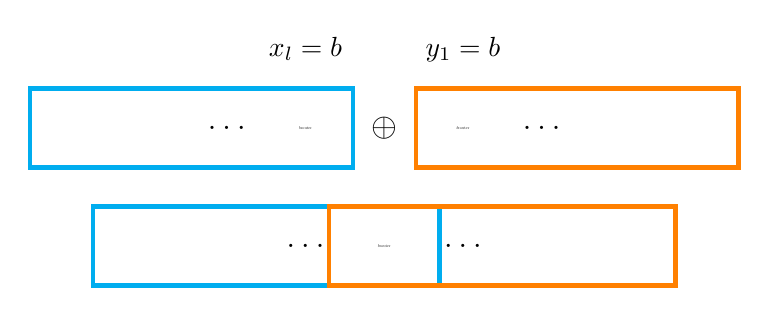
\begin{tikzpicture}
\draw[cyan, ultra thick] (-3.5, -0.5) rectangle (0.6, 0.5);
\draw[orange, ultra thick] (1.4, -0.5) rectangle (5.5, 0.5);

\node[scale=0.15] (v) at (0, 0) {\router{$b$}{router}};
\node[scale=0.15] (u) at (2, 0) {\router{$b$}{router}};
\node at (0, 1) {$x_l = b$};
\node at (2, 1) {$y_{1} = b$};
\node[left of=v] {\large $\ldots$};
\node[right of=u] {\large $\ldots$};

\node at (1, 0) {\large $\oplus$};
\node[rotate=-90] at (1, -0.75) {\large $\rightarrowtail$};

\node[scale=0.15] (b) at (1, -1.5) {\router{$b$}{router}};
\node[left of=b] {\large $\ldots$};
\node[right of=b] {\large $\ldots$};

\draw[cyan, ultra thick] (-2.7, -2) rectangle (1.7, -1);
\draw[orange, ultra thick] (0.3, -2) rectangle (4.7, -1);

\end{tikzpicture}
\\[0.25cm]
\emph{Case 1:} $x_l = y_1 = b \in V$
\\[1cm]
\begin{tikzpicture}
\draw[cyan, ultra thick] (-3.5, -0.5) rectangle (0.6, 0.5);
\draw[orange, ultra thick] (1.4, -0.5) rectangle (5.5, 0.5);

\node[scale=0.15] (v) at (0, 0) {\router{$b$}{router}};
\node[scale=0.15] (u1) at (2, 0) {\router{$b$}{router}};
\node[scale=0.15] (u2) at (4, 0) {\router{$*$}{router}};
\draw[line width=2]  (u1) edge[above, sloped] node[black,font=\bfseries] (l) {} (u2);
\draw (u1) edge[line width=4, darkgreen, above, ->, dotted] (u2);
\node at (0, 1) {$x_l = b$};
\node at (3, 1) {$y_1 = (b, *)$};
\node at (1, 0) {\large $\oplus$};

\node[left of=v] {\large $\ldots$};
\node[right of=u2] {\large $\ldots$};
\node[rotate=-90] at (3, -0.75) {\large $\rightarrowtail$};

\node[scale=0.15] (x) at (3, -1.5) {\router{$*$}{router}};
\node[scale=0.15] (b) at (1, -1.5) {\router{$b$}{router}};
\node[left of=b] {\large $\ldots$};
\node[right of=x] {\large $\ldots$};
\draw[line width=2] (b) edge[above, sloped] (x);
\draw (b) edge[line width=4, darkgreen, above, ->, dotted] (x);

\draw[cyan, ultra thick] (-2.7, -2) rectangle (1.7, -1);
\draw[orange, ultra thick] (0.3, -2) rectangle (4.7, -1);

\end{tikzpicture}
\\[0.25cm]
\emph{Case 2:} $x_l \in E(G)$, $y_{1} \in V(G)$ and $x^2_l =  y_1 = b$
\\[1cm]
\begin{tikzpicture}
\draw[cyan, ultra thick] (-1.5, -0.5) rectangle (2.6, 0.5);
\draw[orange, ultra thick] (3.4, -0.5) rectangle (7.5, 0.5);

\node[scale=0.15] (v1) at (0, 0) {\router{$x$}{router}};
\node[scale=0.15] (v2) at (2, 0) {\router{$b$}{router}};
\node[scale=0.15] (u) at (4, 0) {\router{$b$}{router}};
\draw[line width=2]  (v1) edge[above, sloped] node[black,font=\bfseries] (l) {} (v2);
\draw (v1) edge[line width=4, darkgreen, above, ->, dotted] (v2);
\node at (1, 1) {$x_l = (*, b)$};
\node at (4, 1) {$y_1 = b$};
\node at (3, 0) {\large $\oplus$};

\node[left of=v1] {\large $\ldots$};
\node[right of=u] {\large $\ldots$};
\node[rotate=-90] at (3, -0.75) {\large $\rightarrowtail$};

\node[scale=0.15] (x) at (1, -1.5) {\router{$x$}{router}};
\node[scale=0.15] (b) at (3, -1.5) {\router{$b$}{router}};
\node[left of=x] {\large $\ldots$};
\node[right of=b] {\large $\ldots$};
\draw[line width=2] (x) edge[above, sloped] (b);
\draw (x) edge[line width=4, darkgreen, above, ->, dotted] (b);
\draw[cyan, ultra thick] (-0.5, -2) rectangle (3.7, -1);
\draw[orange, ultra thick] (2.3, -2) rectangle (6.5, -1);

\end{tikzpicture}
\\[0.25cm]
\emph{Case 3:} $x_l \in V(G)$, $y_1 \in E(G)$ and $x_l = y^1_1 = b$
\\[1cm]
\begin{tikzpicture}
\draw[cyan, ultra thick] (-1.5, -0.5) rectangle (2.6, 0.5);
\draw[orange, ultra thick] (3.4, -0.5) rectangle (7.5, 0.5);

\node[scale=0.15] (v1) at (0, 0) {\router{$*$}{router}};
\node[scale=0.15] (v2) at (2, 0) {\router{$b$}{router}};
\node[scale=0.15] (u1) at (4, 0) {\router{$b$}{router}};
\node[scale=0.15] (u2) at (6, 0) {\router{$*$}{router}};
\draw[line width=2]  (v1) edge[above, sloped] node[black,font=\bfseries] (l) {} (v2);
\draw (v1) edge[line width=4, darkgreen, above, ->, dotted] (v2);
\draw[line width=2]  (u1) edge[above, sloped] node[black,font=\bfseries] (l) {} (u2);
\draw (u1) edge[line width=4, darkgreen, above, ->, dotted] (u2);
\node at (1, 1) {$x_l = (*, b)$};
\node at (5, 1) {$y_1 = (b, *)$};
\node at (3, 0) {\large $\oplus$};
\node[left of=v1] {\large $\ldots$};
\node[right of=u2] {\large $\ldots$};

\node[rotate=-90] at (3, -0.75) {\large $\rightarrowtail$};

\node[scale=0.15] (x) at (1, -1.5) {\router{$*$}{router}};
\node[scale=0.15] (b) at (3, -1.5) {\router{$b$}{router}};
\node[scale=0.15] (y) at (5, -1.5) {\router{$*$}{router}};
\node[left of=x] {\large $\ldots$};
\node[right of=y] {\large $\ldots$};
\draw[line width=2] (x) edge[above, sloped] (b);
\draw[line width=2] (b) edge[above, sloped] (y);
\draw (x) edge[line width=4, darkgreen, above, ->, dotted] (b);
\draw (b) edge[line width=4, darkgreen, above, ->, dotted] (y);

\draw[cyan, ultra thick] (-0.5, -2) rectangle (3.7, -1);
\draw[orange, ultra thick] (2.3, -2) rectangle (6.5, -1);


\end{tikzpicture}
\\[0.25cm]
\emph{Case 4:} $x_l \in E(G)$, $y_1 \in E(G)$ and $x^2_l = y^1_1 = b$
\end{tabular}
\end{center}
\caption{The four cases of sr-path concatenation.}
\label{fig:sr-concat}
\end{figure}

In contrast with sr-path addition, the cost of the resulting sr-path after a concatenation
will depend on the types of the segments at the end of the first path and at the start 
of the second.

\begin{lemma}
\label{lemma:concat-cost}
Let $G$ be a network and $\sr{p} = \langle x_1, \ldots, x_l \rangle$ be a sr-path from
$a$ to $b$ and $\sr{q} = \langle y_1, \ldots, y_r \rangle$ be a sr-path from $b$ to $c$, where $a, b, c \in V(G)$.
Then
\[ \cost(\sr{p} \oplus \sr{q}) =
  \begin{cases}
    \cost(\sr{p}) + \cost(\sr{q}) & \quad \text{if } x_l \in E(G) \text{ and } y_1 \in E(G) \\
    \cost(\sr{p}) + \cost(\sr{q}) - 1 & \quad \text{otherwise} \\
  \end{cases}
\]
\end{lemma}

\begin{proof}
If $x_l \in E(G)$ and $y_1 \in E(G)$ then $\sr{p} \oplus \sr{q} = \sr{p} + \sr{q}$ so the result comes from 
Lemma \ref{lemma:srsumcost}. Otherwise, in each case $\sr{p} \oplus \sr{q}$ has the same elements as $\sr{p} + \sr{q}$ except
that we removed a node segment with cost $1$. Thus, by Lemma \ref{lemma:srsumcost}, we have that
$$
\cost(\sr{p} \oplus \sr{q}) = \cost(\sr{p} + \sr{q}) - 1 = \cost(\sr{p}) + \cost(\sr{q}) - 1
$$
\end{proof}

These operations will be important later on because a lot of algorithms for solving problems related to segment routing
can be expressed as dynamic programs where the solution sr-path is built upon smaller sr-paths. These properties tell
use how the segment cost of the paths is affected by these operations.

It is often useful to refer to the set of nodes and edges that belong to some path represented by a sr-path leading
to the following definition.

\begin{definition}
Let $G$ be a network and $\sr{p} = \langle x_1, \ldots, x_l \rangle$ a sr-path on $G$. We define the set of nodes in $\sr{p}$ as
$$
V(\sr{p}) = \bigcup_{i = 1}^l \{x^1_i, x^2_i \} \quad \cup \quad \bigcup_{i = 2}^l V(\sp(x^2_{i - 1}, x^1_i))
$$
We define the set of edges of $\sr{p}$ as
$$
E(\sr{p}) = \left\{ x_i \mid \textrm{$x_i$ is an adjacency segment} \right\} \quad \cup \quad \bigcup_{i = 2}^l E(\sp(x^2_{i - 1}, x^1_i))
$$
\end{definition}

\begin{definition}
Let $G$ be a network and $\sr{p}$ be a sr-path on $G$. We call the subgraph $(V(G), E(\sr{p}))$ the \emph{forwarding
subnetwork} of $\sr{p}$ and denote it by $\forw(\sr{p})$. We write the set of edge in the forwarding graph as
$E(\forw(\sr{p})) = E(\sr{p})$. We can easily see that if $\sr{p} = \langle x_1, \ldots, x_l \rangle$ then
$$
E(\sr{p}) = \bigcup_{i = 2} E(\sp(x^2_{i - 1}, x^1_i)) \cup \bigcup{i : x_i \in E(G)} x_i.
$$
\end{definition}

To lighten the notation, we often omit the parenthesis and write $\forw \langle x_1, \ldots, x_l \rangle$ rather than
$\forw(\langle x_1, \ldots, x_l \rangle)$.

The forwarding subnetwork of a sr-path $\sr{p}$ encodes every path on which packets might travel when forwarded over $\sr{p}$.
However it does not encode how many times a given link is traversed by the sr-path because each edge that is traversed by $\sr{p}$ 
appears exactly once.

\begin{definition}
Let $G$ be a network and $\sr{p} = \langle x_1, \ldots, x_l \rangle$ be a sr-path on $G$. We say that $\sr{p}$ is \emph{deterministic} if and only if
for each $i \in \{2, \ldots, l\}$, there exists a unique shortest path between $x^2_{i - 1}$ and $x^1_i$.
\end{definition}

Deterministic sr-paths are important when we want to have guarantees about the set of links that are traversed
when one uses SR to forward traffic over a given sr-path. Because there exists a single shortest path between any two consecutive endpoints,
they never use ECMP. For this reason they map back to a unique path on the network $G$. This kind of paths will be important in Chapter \ref{chapter:scmon}
where we design an algorithm that leverages segment routing to provide network monitoring for detecting single link failures. In this context,
we will need to know exactly which links are covered by each sr-path used for the monitoring.

Another application of deterministic sr-paths, which we will tackle in the next section, is the reverse problem, where we start from a path on $G$
and we want to find a sr-path whose forwarding graph matches that path.

\begin{lemma}
\label{lemma:deterministic-concat}
Let $G$ be a network and $\sr{p}$ be a deterministic sr-path from
$a$ to $b$ and $\sr{q}$ be a deterministic sr-path from $b$ to $c$ 
then $\sr{p} \oplus \sr{q}$ is a deterministic sr-path
from $a$ to $c$.
\end{lemma}

\begin{proof}
The fact that $\sr{p} \oplus \sr{q}$ is well defined is simply because we assumed
that $\sr{p}$ is a sr-path from $a$ to $b$ and $\sr{q}$ a sr-path from $b$ to $c$. 
It remains to show that it is deterministic.

Write $\sr{p} = \langle x_1, \ldots, x_l \rangle$ and 
$\sr{q} = \langle y_1, \ldots, y_r \rangle$.
Let $z_i, z_{i + 1}$ be consecutive elements of $\sr{p} \oplus \sr{q}$. 
We need to prove that
there exists a unique shortest path between $z^2_i$ and $z^1_{i + 1}$.
If both $z_i, z_{i + 1}$ belong to $\sr{p}$ or $\sr{q}$ then this is true since both
$\sr{p}$ and $\sr{q}$ are deterministic. Otherwise, there are four cases that we need
to consider.

\emph{Case 1:} $x_l = y_1$ are both node segments. In this case we know that
$\sr{p} \oplus \sr{q} = \langle x_1, \ldots, x_l, y_2, \ldots, y_r \rangle$.
Thus, $z_i = x_l = y_1$ and $z_{i + 1} = y_2$. Hence, since $\sr{q}$ is deterministic,
there exists a unique shortest path between $z^2_i = y^2_1$ and $z^1_{i + 1} = y^1_2$.

\emph{Case 2:} $x_l,  y_1$ are both adjacency segments and 
$x^2_l = y^1_1$. In this case we know that
$\sr{p} \oplus \sr{q} = \langle x_1, \ldots, x_l, y_1, y_2, \ldots, y_r \rangle$.
Hence, $z_i = x_l$ and $z_{i + 1} = y_1$ so $z^2_i = x^2_l = y^1_1 = z^1_{i + 1}$ so
the unique shortest path between $z^2_i$ and $z^1_{i + 1}$ is the empty path.

\emph{Case 3:} $x_l$ is an adjacency segment and $y_1$ is a node segment such that
$x^2_l = y_1$. By definition, 
$\sr{p} \oplus \sr{q} = \langle x_1, \ldots, x_l, y_2, \ldots, y_r \rangle$.
Thus, $z_i = x_l$ and $z_{i + 1} = y_2$. Thus, since $\sr{q}$ is deterministic,
there exists a unique shortest path between $z^2_i = x^2_l = y^2_1$ and $z^1_{i + 1} = y^1_2$.

\emph{Case 4:} $x_l$ is a node segment and $y_1$ is an adjacent segment such that
$y^1_1 = x_l$. Therefore $\sr{p} \oplus \sr{q} = \langle x_1, \ldots, x_{l - 1}, y_1, y_2, \ldots, y_r \rangle$.
Thus, $z_i = x_{l - 1}$ and $z_{i + 1} = y_1$. Thus, since $\sr{p}$ is deterministic,
there exists a unique shortest path between $z^2_i = x^2_{l - 1}$ and $z^1_{i + 1} = y^1_2 = x^1_l$.
\end{proof}

\section{Acyclic sr-paths}
\label{section:acyclic}

Sr-paths can contain cycles as shown in Figure \ref{fig:cyclicsr}. In some situations we can take advantage of these
cycles to obtain better solution. We discuss one such example when we talk about traffic engineering in Chapter \ref{chapter:te}. 
In other situations we can show that cycles can never lead to an optimal solution.
We are now going to prove that we can always transform a sr-path that contains cycles into a sr-path that is acyclic,
visits a subset of the edges previously visited and does not have a higher segment cost. 
In the case of Figure \ref{fig:cyclicsr} we could achieve this by replacing node segment $\node{d}$ by $\node{e}$.
The set of edges in $\forw \langle \node{a}, \node{b}, \node{e}, \node{f} \rangle$ is a subset of the set of edges 
in $\forw \langle \node{a}, \node{b}, \node{d}, \node{f} \rangle$ but $\langle \node{a}, \node{b}, \node{e}, \node{f} \rangle$
is acyclic.

\begin{figure}[H]
\begin{center}
\begin{tikzpicture}
\def\x{0}
\def\y{0}
\node[scale=0.15] (a) at (0.5 + \x,  0.5 + \y) {\router{a}{marked}};
\node[scale=0.15] (b) at (0.5 + \x, -1.0 + \y) {\router{b}{marked}};
\node[scale=0.15] (c) at (2.5 + \x,  0.0 + \y) {\router{c}{router}};
\node[scale=0.15] (d) at (4.5 + \x,  0.0 + \y) {\router{d}{marked}};
\node[scale=0.15] (e) at (4.0 + \x, -2.0 + \y) {\router{e}{router}};
\node[scale=0.15] (g) at (6.0 + \x,  0.5 + \y) {\router{g}{router}};
\node[scale=0.15] (i) at (8.0 + \x,  0.0 + \y) {\router{i}{router}};
\node[scale=0.15] (h) at (7.0 + \x, -1.5 + \y) {\router{h}{router}};
\node[scale=0.15] (f) at (4.0 + \x, -3.5 + \y) {\router{f}{marked}};
\node[scale=0.15] (j) at (8.0 + \x, -2.5 + \y) {\router{j}{router}};
\draw[line width=2] (f) edge[above, sloped] node[black,font=\bfseries] {\tiny \texttt{}} (j);
\draw[line width=2] (h) edge[above, sloped] node[black,font=\bfseries] {\tiny \texttt{}} (j);
\draw[line width=2] (a) edge[above, sloped] node[black,font=\bfseries] {\tiny \texttt{}} (b);
\draw[line width=2] (b) edge[above, sloped] node[black,font=\bfseries] {\tiny \texttt{}} (c);
\draw[line width=2] (b) edge[above, sloped] node[black,font=\bfseries] {\tiny \texttt{}} (e);
\draw[line width=2] (b) edge[above, sloped] node[black,font=\bfseries] {\tiny \texttt{}} (f);
\draw[line width=2] (e) edge[above, sloped, bend left=10] node[black,font=\bfseries] {\tiny \texttt{}} (f);
\draw[line width=2] (e) edge[above, sloped, bend right=10] node[black,font=\bfseries] {\tiny \texttt{}} (f);
\draw[line width=2] (h) edge[above, sloped] node[black,font=\bfseries] {\tiny \texttt{}} (f);
\draw[line width=2] (g) edge[above, sloped] node[black,font=\bfseries] {\tiny \texttt{}} (i);
\draw[line width=2] (i) edge[above, sloped] node[black,font=\bfseries] {\tiny \texttt{}} (h);
\draw[line width=2]  (d) edge[above, sloped] node[black,font=\bfseries] {\tiny \texttt{}} (g);
\draw[line width=2]  (d) edge[above, sloped] node[black,font=\bfseries] {\tiny \texttt{}} (e);
\draw[line width=2]  (e) edge[above, sloped] node[black,font=\bfseries] {\tiny \texttt{}} (h);
\draw[line width=2]  (g) edge[above, sloped] node[black,font=\bfseries] {\tiny \texttt{}} (h);
\draw[line width=2]  (c) edge[above, sloped] node[black,font=\bfseries] {\tiny \texttt{}} (d);
\draw[line width=2]  (a) edge[above, sloped] node[black,font=\bfseries] {\tiny \texttt{}} (b);
\draw[line width=2]  (a) edge[above, sloped] node[black,font=\bfseries] {\tiny \texttt{}} (c);

%%%%
\draw (a) edge[line width=3, darkgreen, above, ->, bend right = 10] (b);
\draw (b) edge[line width=3, darkgreen, above, ->, bend right = 10] (c);
\draw (b) edge[line width=3, darkgreen, above, ->, bend left = 10] (e);
\draw (c) edge[line width=3, darkgreen, above, ->, bend right = 10] (d);
\draw (e) edge[line width=3, darkgreen, above, ->, bend right = 20] (d);
\draw (d) edge[line width=3, darkgreen, above, ->, bend right = 20] (e);
\draw (e) edge[line width=3, darkgreen, above, ->, bend left = 20] (f);
\draw (e) edge[line width=3, darkgreen, above, ->, bend right = 20] (f);

\draw (a) edge[line width=3, orange, above, ->, bend left = 10] (b);
\draw (b) edge[line width=3, orange, above, ->, bend left = 10] (e);

\draw (e) edge[line width=3, orange, above, ->, bend left = 40] (f);
\draw (e) edge[line width=3, orange, above, ->, bend right = 40] (f);



\node[left = 0.1cm of a, draw, fill=green] (x1) {\footnotesize $x_1$};
\node[left = 0.1cm of b, draw, fill=green] (x2) {\footnotesize $x_2$};
\node[above = 0.1cm of d, draw, fill=green] (x3) {\footnotesize $x_3$};
\node[below = 0.1cm of f, draw, fill=green] (x4) {\footnotesize $x_4$};

\node[left = 0.1cm of x1, draw, fill=orange!20!white] (y1) {\footnotesize $y_1$};
\node[left = 0.1cm of x2, draw, fill=orange!20!white] (y2) {\footnotesize $y_2$};
\node[left bottom = 0.1cm of e, draw, fill=orange!20!white] (y3) {\footnotesize $y_3$};
\node[left = 0.1cm of x4, draw, fill=orange!20!white] (y4) {\footnotesize $y_4$};

\end{tikzpicture}
\end{center}
\caption{Illustration of a cyclic sr-path $\sr{p} = \langle \node{a}, \node{b}, \node{d}, \node{f} \rangle$. It contains
cycle $(\edge{d}{e}, \edge{e}{d})$. The sr-path $\sr{q} = \langle \node{a}, \node{b}, \node{e}, \node{f} \rangle$ also goes
from $\node{a}$ to $\node{f}$ but is acyclic. It visits a subset of the edges of $\forw(\sr{p})$ so it is a sr-subpath
of $\sr{q}$.}
\label{fig:cyclicsr}
\end{figure}

Next we give a formal definition of cyclic sr-paths. 

\begin{definition}
Let $G$ be a network and $\sr{p}$ a sr-path on $G$. We say that $\sr{p}$ is \emph{cyclic} if $\forw(\sr{p})$ is
cyclic.
\end{definition}

Do not confuse this definition with sr-cycles. A sr-cycle is simply a sr-path whose first and last nodes are the same.
Of course any sr-cycle is cyclic. But not all cyclic sr-paths are sr-cycles. We start by proving the theorem in the case
where the sr-path contains only node segments.

The following simple lemma shows that if two nodes are connected then we can always find an acyclic sr-path between them.

\begin{lemma}
Let $G$ be a network and $u, v \in G$. If there exists a path from $u$ to $v$ on $G$ then there exists an acyclic sr-path
from $u$ to $v$.
\end{lemma}

\begin{proof}
We can simply take a minimal segmentation $\sr{p}$ of $p$. In this case $\forw(\sr{p}) = p$ so it is acyclic.
\end{proof}

\begin{definition}
Let $G$ be a network and $\sr{p}$ a sr-path from $u$ to $v$ on $G$. We say that $\sr{q}$ is a \emph{sr-subpath} of $\sr{p}$ if 
$\sr{q}$ is a sr-path from $u$ to $v$ and $\forw(\sr{q})$ is a subnetwork of $\forw(\sr{p})$.
\end{definition}

The next theorem shows that for any sr-path, we can always find a sr-subpath of it that is acyclic and whose segment
cost is at most the segment cost of the original path. This theorem has important practical implications as we will
see in Chapter \ref{chapter:disjoint}.

\begin{theorem}
\label{thm:sracyclic_noadj}
Let $G$ be a network with $\igp(e) > 0$ for all $e \in E(G)$, $u, v \in V(G)$ with $u \neq v$ and $\sr{p}$ be a sr-path on $G$ from $u$ to $v$ using only node segments. 
Then there exists an acyclic sr-path $\sr{q}$ from $u$ to $v$
such that $\forw(\sr{q}) \subseteq \forw(\sr{p})$ and $\cost(\sr{q}) \leq \cost(\sr{p})$.
\end{theorem}

\begin{proof}
Let $\sr{p} = \langle x_1, \ldots, x_n \rangle$. The proof is by induction on $n$. If $n = 1$
then $\forw(\sr{p})$ has 0 edges and is therefore acyclic. If $n = 2$ then $\forw(\sr{p})$ is equal to the
union of shortest paths from $x_1$ to $x_2$ which form an acyclic graph.
Assume that $\langle x_1, \ldots, x_{n - 1} \rangle$ is acyclic but $\sr{p}$ is not. We will show
how to construct $\sr{q}$ satisfying the theorem conditions.

Since $\sr{p}$ is cyclic, we can let $i$ be the smallest index such that
there exists a node $v$ in $\forw \langle x_i, x_{i + 1} \rangle$ that belongs to a cycle in $\forw(\sr{p})$.
If several such nodes exist, assume that $v$ is the one closest to $x_i$ (in terms of IGP, if several exist, choose any).

Let $\sr{q} = \langle x_1, \ldots, x_i, v, x_n\rangle$. Since $v$ belongs to both $\forw \langle x_i, x_{i + 1} \rangle$ and
$\forw \langle x_{n - 1}, x_n \rangle$ we have
$$
\forw \langle x_1, \ldots, x_i, v \rangle \subseteq \forw \langle x_1, \ldots, x_i, x_{i + 1} \rangle
$$
and
$$
\forw \langle v, x_n \rangle \subseteq \forw \langle x_{n - 1}, x_n \rangle
$$
so that
\begin{align*}
\forw(\sr{q}) & = \forw \langle x_1, \ldots, x_i, v \rangle \cup \forw \langle v, x_n \rangle \\
              & \subseteq \forw \langle x_1, \ldots, x_i, x_{i + 1} \rangle \cup \forw \langle x_{n - 1}, x_n \rangle \\
              & \subseteq \forw \langle x_1, \ldots, x_i, x_{i + 1} \rangle \cup \forw \langle x_{i + 2}, \ldots x_{n - 2} \rangle \cup \forw \langle x_{n - 1}, x_n \rangle \\
              & = \forw(\sr{p}).
\end{align*}
Similarly, we have
\begin{align*}
\cost(\sr{q}) & = \cost \langle x_1, \ldots, x_i, v \rangle + \cost \langle v, x_n \rangle - 1 \\
              & = \cost \langle x_1, \ldots, x_i, x_{i + 1} \rangle + \cost \langle x_{n - 1}, x_n \rangle - 1 \\
              & < \cost \langle x_1, \ldots, x_i, x_{i + 1} \rangle + \cost \langle x_{i + 2}, \ldots x_{n - 2} \rangle + \cost \langle x_{n - 1}, x_n \rangle \\
              & = \cost(\sr{p}).
\end{align*}
The sr-path $\sr{q}$ starts at $x_1 = u$ and ends at $x_n = v$. If $\sr{q}$ is acyclic then the proof is complete. Otherwise, let $c$
by a cycle on $\forw(\sr{q})$. Since both $\forw \langle x_1, \ldots, x_i, v \rangle$ and $\forw \langle v, x_n \rangle$ are acyclic,
$c$ cannot be fully contained in either one of them. This means that there must be a node $u \in V(c) \setminus v$ in 
$\forw \langle x_1, \ldots, x_i, v \rangle$. By choice of $v$, the distance from $x_i$ to $u$ and $v$ must be the same and $u$ must be
in the shortest path from $x_i$ to $v$. This is impossible since we assume that $\igp(e) > 0$ for all $e \in E(G)$.
\end{proof}

The theorem is also true in the general case where we allow the sr-path $\sr{p}$ to contain adjacency segments. However the proof is
quite tedious as it involves a lot of cases. Rather than provide a detailed proof, we instead provide the case analysis and a valid
acyclic sr-subpath in each case.

The construction works very similarly as in the proof of Theorem \ref{thm:sracyclic_noadj}. Let's focus on the general case
only. Assume that $\sr{p} = \langle x_1, \ldots, x_n \rangle$ is cyclic but $\langle x_1, \ldots, x_{n - 1} \rangle$ is acyclic. 
As in the above proof, let $i$ be the smallest index such that
there exists a node $v$ in $\forw \langle x_i, x_{i + 1} \rangle$ that belongs to a cycle in $\forw(\sr{p})$.
If several such nodes exist, assume that $v$ is the one closest to $x_i$ (in terms of IGP, if several exist, choose any).

With this choice of $x_i$ and $v$ we can build $\sr{q}$ by following Table \ref{tab:cases}. The construction of $\sr{q}$ depends on
two things:

\begin{enumerate}
 \item Where $v$ is crossed when we move on $\sr{p}$ from $x_i$ to $x_{i + 1}$.
 \item Where $v$ is crossed when we move on $\sr{p}$ from $x_{n - 1}$ to $x_n$.
\end{enumerate}

For the first, we consider three cases: (1) $v$ is the node $x^1_i$, (2) $v$ is the node $x^2_{i}$ or (3) $v$ is neither
of those nodes and belongs to a shortest path from $x^2_i$ to $x^1_{i + 1}$ (we represent this by $v \in \langle x^2_i, x^1_{i + 1} \rangle$
on the table). This is represented the columns of the table.

For the second, we consider five cases: (1) $v$ is the node $x^1_{n - 1}$, (2) $v$ is the node $x^2_{n - 1}$, (3) $v$ is the node $x^1_n$, 
(4) $v$ is the node $x^2_n$ and finally (5) $v$ is neither of those nodes and belongs the shortest path between $x^2_{n - 1}$ to $x^1_n$ 
(we represent this by $v \in \langle x^2_{n - 1}, x^1_n\rangle$ on the table). These cases are represented by the rows of the table.

For example, if $v = x^2_i$ and $v \in \langle x_{n - 1}, x_, \rangle$ then $\sr{q} = \langle x_1, \ldots, x_i, x_n \rangle$ is a 
solution.

Note that for construction to be correct we do not need to assume anything about the kind of segments $x_i$, $x_{i + 1}$, $x_{n-1}$ and
$x_n$ are. It may seem that we are assuming that they are adjacency segments but if they are not the construction still works. The only
thing that might happen is that we may have some repeated redundant segments in $\sr{q}$. However even with these, we can show that 
$\cost(\sr{q}) \leq \cost(\sr{p})$.

\begin{center}
\begin{table}
\footnotesize
\begin{tabular}{c|ccccc}
                                       & $v = x^1_i$ & $v = x^2_i$ & $v \in \langle x^2_i, x^1_{i + 1} \rangle$ \\[0.1cm]
                                       \midrule
$v = x^1_{n - 1}$                      & $\langle x_1, \ldots, x_{i-1}, x_{n - 1}, x_n \rangle$ 
                                       & $\langle x_1, \ldots, x_i, x_{n - 1}, x_n \rangle$ 
                                       & $\langle x_1, \ldots, x_i, x_{n - 1}, x_n \rangle$      \\[0.05cm]
                                       
$v = x^2_{n - 1}$                      & $\langle x_1, \ldots, x_{i-1}, v, x_n \rangle$ 
                                       & $\langle x_1, \ldots, x_{i}, x_n \rangle$ 
                                       & $\langle x_1, \ldots, x_{i}, v, x_n \rangle$    \\[0.05cm]
                                       
                                       
$v = x^1_n$                            & $\langle x_1, \ldots, x_{i-1}, x_n \rangle$ 
                                       & $\langle x_1, \ldots, x_i, x_n \rangle$
                                       & $\langle x_1, \ldots, x_i, v, x_n \rangle$   \\[0.05cm]
                                       
$v = x^2_n$                            & $\langle x_1, \ldots, x_{i-1}, v \rangle$ 
                                       & $\langle x_1, \ldots, x_i \rangle$
                                       & $\langle x_1, \ldots, x_i, v \rangle$  \\[0.05cm]
                                       
$v \in \langle x_{n - 1}, x_n \rangle$ & $\langle x_1, \ldots, x_{i-1}, v, x_n \rangle$ 
                                       & $\langle x_1, \ldots, x_i, x_n \rangle$
                                       & $\langle x_1, \ldots, x_i, v, x_n \rangle$
\end{tabular}
\caption{Construction of an acyclic sr-subpath.}
\label{tab:cases}
\end{table}
\end{center}

Putting these ideas together we can prove the following² general theorem.

\begin{theorem}
\label{thm:sracyclic}
Let $G$ be a network with $\igp(e) > 0$ for all $e \in E(G)$, $u, v \in V(G)$ with $u \neq v$ and $\sr{p}$ be a sr-path on $G$ from $u$ to $v$. Then there exists an acyclic sr-path $\sr{q}$ from $u$ to $v$
such that $\forw(\sr{q}) \subseteq \forw(\sr{p})$ and $\cost(\sr{q}) \leq \cost(\sr{p})$.
\end{theorem}


% \begin{theorem}
% \label{thm:sracyclic_node}
% Let $G$ be a network, $u, v \in V(G)$ with $u \neq v$ and $\sr{p}$ be a sr-path on $G$ from $u$ to $v$ containing only node segments. Then there exists an acyclic sr-path $\sr{q}$ from $u$ to $v$
% such that $\forw(\sr{q}) \subseteq \forw(\sr{p})$ and $\cost(\sr{q}) \leq \cost(\sr{p})$.
% \end{theorem}
% 
% \begin{proof}
% If $\sr{p} = \langle x_1, x_2 \rangle$ then $\forw(\sr{p}) = \sp(x_1, x_2)$ and thus it is acyclic by Lemma \ref{lemma:dag}.
% 
% To give some intuition about the general case we start by proving the result for $n = 3$. 
% Suppoe now that $\sr{p} = \langle x_1, x_2, x_3 \rangle$. If $\sr{p}$ is acyclic then
% there is nothing to prove since we can just take $\sr{q} = \sr{p}$. Otherwise, Let $y$ be a node such that $\dist(x_1, y)$ is minimal
% and $y$ belongs to a cycle in $\forw(\sr{p})$. Let $\sr{q} = \langle x_1, y, x_3 \rangle$. Suppose that there is a cycle in
% $\forw(\sr{q})$. Let $z$ be a node that is visited more than once in that cycle. Since $\langle x_1, y \rangle$ and $\langle y, x_3 \rangle$ are
% both acyclic we know that $z \neq y$. Therefore, $y$ must occur on a path from $x_1$ to $y$ and also on a path from $y$ to $x_3$. Hence,
% $d(x_1, z) < d(x_1, y)$. On the other hand, $E(\sp(x_1, y)) \subseteq E(\sp(x_1, x_2))$ and $E(\sp(y, x_3)) \subseteq E(\sp(x_1, x_3))$ so 
% $\forw(\sr{q}) \subseteq \forw(\sr{p})$. Thus, in particular, $z$ is also a node in a cycle in $\forw(\sr{p})$ contradicting the choice of $y$ since $d(x_1, z) < d(x_1, y)$.
% We conclude that $\forw(\sr{q})$ is acyclic. Figure
% \ref{fig:acyclicproof1} illustrates this.
% Clearly $\cost(\sr{p}) = \cost(\sr{q})$ since $\cost(y) = \cost(x_2)$ because $y$ is a node segment.
% 
% \begin{figure}
% \begin{center}
% \begin{tabular}{ccc}
% \begin{tikzpicture}[scale = 0.8]
% \draw[white] (-1, -1) rectangle (5, 5);
% \node[scale=0.15] (x1) at (0, 0) {\router{$x_1$}{router}};
% \node[scale=0.15] (x2) at (4, 0) {\router{$x_2$}{router}};
% \node[scale=0.15] (x3) at (2, 4) {\router{$x_3$}{router}};
% 
% 
% \node[scale=0.15] (y) at (2, 2) {\router{$y$}{router}};
% 
% \draw[line width=2, black] (x1) edge[below, sloped, bend left, dashed, ->] (y);
% \draw[line width=2, black] (y) edge[below, sloped, bend left, dashed, ->] (x2);
% 
% \draw[line width=2, black] (y) edge[below, sloped, bend left, dashed, ->] (x3);
% \draw[line width=2, black] (x2) edge[below, sloped, bend left, dashed, ->] (y);
% 
% \end{tikzpicture}
% 
% &
% 
% \begin{tikzpicture}[scale = 0.8]
% \draw[white] (-1, -1) rectangle (1, 5);
% \node at (0, 2) {$\rightarrow$};
% \end{tikzpicture}
% &
% 
% \begin{tikzpicture}[scale = 0.8]
% \draw[white] (-1, -1) rectangle (3, 5);
% 
% \node[scale=0.15] (x1) at (0, 0) {\router{$x_1$}{router}};
% \node[scale=0.15] (x3) at (2, 4) {\router{$x_3$}{router}};
% 
% 
% \node[scale=0.15] (y) at (2, 2) {\router{$y$}{router}};
% 
% \draw[line width=2, black] (x1) edge[below, sloped, bend left, dashed, ->] (y);
% 
% \draw[line width=2, black] (y) edge[below, sloped, bend left, dashed, ->] (x3);
% 
% \end{tikzpicture}
% 
% \\
% 
% $\langle x_1, x_2, x_3 \rangle$ & & $\langle x_1, y, x_3 \rangle$
% 
% \end{tabular}
% \end{center}
% \caption{Illustration of the proof for $\sr{p} = \langle x_1, x_2, x_3 \rangle$.}
% \label{fig:acyclicproof1}
% \end{figure}
% 
% For the general case write $\sr{p} = \langle x_1, \ldots, x_n \rangle$. If $\sr{p}$ is acyclic then chose $\sr{q} = \sr{p}$.
% Otherwise let $y$ a the node that appears in a cycle such that $\dist(x_1, y)$ is minimal. Let $i$ be the smallest index
% such that there exists a shortest path from $x_i$ to $x_{i + 1}$ passing by $y$ and $j$ be the largest such index.
% Let $\sr{q} = \langle x_1, \ldots, x_{i - 1}, y, x_{j + 1}, \ldots, x_n \rangle$. In the same way as before, if there is a 
% cycle in $\forw(\sr{q})$ then there is a node $z \neq y$ that is visited by a shortest path form $x_{i'}$ to $x_{i' + 1}$
% and $x_{j'}$ to $y_{j' + 1}$ with $i' < i - 1$ and $j' \geq j + 1$. This contradicts the choice of $y, i$ and $j$.
% Clearly $\sr{q}$ has lower segment cost so the proof is complete.
% \end{proof}
% 
% We can prove that the results holds even if $\sr{p}$ is allowed to contain both node and adjacency segments giving the following theorem.
% The proof is a bit more technical since adjacency segments behave a little bit differently. For example with adjacency segments it is not 
% true that $\langle x_1, x_2 \rangle$ is acyclic. If $x_1 = x_2$ then node $x_1$ is visited twice as shown in Figure \ref{fig:acyclicproof2}.
% 
% \begin{figure}
% \begin{center}
% \begin{tikzpicture}
% \draw[white] (-1, -1) rectangle (5, 5);
% \node[scale=0.15] (u) at (0, 0) {\router{$u$}{router}};
% \node[scale=0.15] (v) at (3, 0) {\router{$v$}{router}};
% 
% \draw[line width=2, black] (u) edge[below, sloped, ->] (v);
% \draw[line width=2, black] (v) edge[below, bend left = 60, dashed, sloped, ->] (u);
% 
% \draw[cyan, line width=2, ->] plot [smooth] coordinates { (0, 0.5) (3, 0.5) (3.8, 0) (3, -0.75) (1.5, -1.4) (0, -0.75) (0.5, -0.25) (2.8, -0.25)};
% 
% \end{tikzpicture}
% 
% \end{center}
% \caption{Sr-path $\langle x_1, x_1 \rangle$ with $x_1 = (u, v)$.}
% \label{fig:acyclicproof2}
% \end{figure}
% 
% 
% \begin{theorem}
% \label{thm:sracyclic}
% Let $G$ be a network, $u, v \in V(G)$ with $u \neq v$ and $\sr{p}$ be a sr-path on $G$ from $u$ to $v$. Then there exists an acyclic sr-path $\sr{q}$ from $u$ to $v$ such that
% $\forw(\sr{q}) \subseteq \forw(\sr{p})$ and $\cost(\sr{q}) \leq \cost(\sr{p})$.
% \end{theorem}
% 
% \begin{proof}
% 
% \end{proof}


\section{Minimal segmentations}

In this section we study the problem of efficiently representing paths in the network with SR.
Suppose that you have a path in your network that you want to use to send traffic between two nodes. Traditional
shortest path routing does not allow you to forward traffic on it unless that path already is a shortest paht with
respect to the $\igp$ weights configured on the links. SR makes it possible, at least in theory, to forward traffic
on \emph{any} path in the network since we can always just add all edges of the path as adjacency segments
in the segment routing stack. In practice however, this solution cannot be implemented because, as we mentioned above, 
due to hardware limitations of the routers currently deployed in the networks, 
the stack size is often limited to a few segments \cite{Tantsura_SID:2017}.

This motivates the problem of, given a path $p$ in the network, finding a sr-path $\sr{p}$ that represents $p$. That is, a sr-path $\sr{p}$
such that if traffic is routed over it, packets will traverse exactly the edges of $p$ in order. To do that, we need a formal definition of what 
does it mean for a sr-path to represent a path in the network.

\begin{definition}
Let $\sr{p} = \langle x_1, \ldots, x_l \rangle$ be a deterministic sr-path. We define
$$
\seq(\sr{p}) = x_1 \oplus \sp(x^2_1, x^1_2) \oplus x_2 \oplus \ldots \oplus \sp(x^2_{l - 1}, x^1_l) \oplus x_l
$$
\end{definition}

Note that since $\sr{p}$ is deterministic, $\seq(\sr{p})$ corresponds to a path in $G$ since each $\sp(x^2_{i - 1}, x^1_i)$
is a single path.

\begin{definition}
Let $G$ be a network and $p$ a path on $G$. A deterministic sr-path $\sr{p} = \langle x_1, \ldots, x_l \rangle$ is said to be a segmentation of $p$ if and only if
$p = \seq(\sr{p})$.
\end{definition}

Note that we restrict ourselves to deterministic sr-paths since the equality in the above definition would never hold if
for some $i$, $\sp(x^2_i, x^1_{i + 1})$ was not a path. Moreover, $\oplus$ is only defined if both operands are paths.
We start by showing that any path possess a segmentation.

\begin{lemma}
\label{lemma:seg_exists}
Let $G$ be a network and $p$ a path on $G$. Then, there exists a sr-path $\sr{p}$ such that $\sr{p}$ is a segmentation of
$p$. Moreover, any path admits a segmentation of cost at most $2|E(G)|$.
\end{lemma}

\begin{proof}
Let $p = (e_1, \ldots, e_l)$ be a path on $G$ and let $\sr{p} = \langle e_1, \ldots, e_l \rangle$. For each $i = 1, \ldots, l - 1$
we have that $\sp(e^2_i, e^1_{i + 1}) = \emptyset$ since $e^2_i = e^1_{i + 1}$. Thus
\begin{align*}
e_1 \oplus \sp(e^2_1, e^1_2) \oplus e_2 \oplus \ldots \oplus \sp(e^2_{l - 1}, e^1_l) \oplus e_l & = e_1 \oplus e_2 \oplus \ldots \oplus e_l = p.
\end{align*}
\end{proof}

Note that previous models of segment routing considered only node segments and therefore this result was not true. In such models it is impossible
to represent some network paths in terms of SR. As we saw in Chapter \ref{chapter:dataset}, there are about $1\%$ of the network links
that do not belong to a shortest path and $24\%$ of pairs of nodes with ECMP. We mentioned that those were the conditions that might lead to the
need of using an adjacency segment. We characterize in Proposition \ref{prop:adj-segs} exactly which situations lead to the need of using
an adjacency segment.

We call the segmentation used in the proof of Lemma \ref{lemma:seg_exists} the \emph{edge segmentation} of $p$.
Consider the path $((\node{a}, \node{b}), (\node{b}, \node{c}), (\node{c}, \node{d}), (\node{d}, \node{g}), (\node{g}, \node{i}))$ shown in green in Figure \ref{fig:min-seg-example}.
We already saw in Lemma \ref{lemma:seg_exists} above that $\sr{p} = \langle (\node{a}, \node{b}), (\node{b}, \node{c}), (\node{c}, \node{d}), (\node{d}, \node{g}), (\node{g}, \node{i}) \rangle$
is a segmentation of $p$. But this is not the unique segmentation of $p$. For example $\sr{q} = \langle \node{a}, (\node{b}, \node{c}), \node{g}, \node{i} \rangle$ is
also a segmentation of $p$. We have
\begin{align*}
e_1 \oplus \sp(e^2_1, e^1_2) \oplus e_2 \oplus \ldots \oplus \sp(e^2_{l - 1}, e^1_l) \oplus e_l & = \\
(\node{a}) \oplus \sp(\node{a}, \node{b}) \oplus (\node{b}, \node{c}) \oplus  \sp(\node{c}, \node{g}) \oplus (g) \oplus \sp(\node{g}, \node{i}) \oplus (i) & = \\
(\node{a}) \oplus ((\node{a}, \node{b})) \oplus ((\node{b}, \node{c})) \oplus  ((\node{c}, \node{d}), (\node{d}, \node{g})) \oplus (g) \oplus ((\node{g}, \node{i})) \oplus (i) & = \\
((\node{a}, \node{b}), (\node{b}, \node{c}), (\node{c}, \node{d}), (\node{d}, \node{g}), (\node{g}, \node{i})).
\end{align*}

\begin{figure}[H]
\begin{center}
\begin{tikzpicture}[scale=1.4]
\def\x{0}
\def\y{0}
\node[scale=0.15] (a) at (0.5 + \x,  0.5 + \y) {\router{a}{marked}};
\node[scale=0.15] (b) at (0.5 + \x, -1.0 + \y) {\router{b}{router}};
\node[scale=0.15] (c) at (2.5 + \x,  0.0 + \y) {\router{c}{router}};
\node[scale=0.15] (d) at (4.5 + \x,  0.0 + \y) {\router{d}{router}};
\node[scale=0.15] (e) at (4.0 + \x, -2.0 + \y) {\router{e}{router}};
\node[scale=0.15] (g) at (6.0 + \x,  0.5 + \y) {\router{g}{marked}};
\node[scale=0.15] (i) at (8.0 + \x,  0.0 + \y) {\router{i}{marked}};
\node[scale=0.15] (h) at (7.0 + \x, -1.5 + \y) {\router{h}{router}};
\draw[line width=2] (a) edge[above, sloped] node[black,font=\bfseries] {\tiny \texttt{}} (b);
\draw[line width=2] (b) edge[above, sloped] node[black,font=\bfseries] {\tiny \texttt{}} (c);
\draw[line width=2] (e) edge[above, sloped] node[black,font=\bfseries] {\tiny \texttt{}} (c);
\draw[line width=2] (b) edge[above, sloped] node[black,font=\bfseries] {\tiny \texttt{}} (e);
\draw[line width=2] (g) edge[above, sloped] node[black,font=\bfseries] {\tiny \texttt{}} (i);
\draw[line width=2] (i) edge[above, sloped] node[black,font=\bfseries] {\tiny \texttt{}} (h);
\draw[line width=2]  (d) edge[above, sloped] node[black,font=\bfseries] {\tiny \texttt{}} (g);
\draw[line width=2]  (d) edge[above, sloped] node[black,font=\bfseries] {\tiny \texttt{}} (e);
\draw[line width=2]  (e) edge[above, sloped] node[black,font=\bfseries] {\tiny \texttt{}} (h);
\draw[line width=2]  (g) edge[above, sloped] node[black,font=\bfseries] {\tiny \texttt{}} (h);
\draw[line width=2]  (c) edge[above, sloped] node[black,font=\bfseries] {\tiny \texttt{}} (d);
\draw[line width=2]  (a) edge[above, sloped] node[black,font=\bfseries] {\tiny \texttt{}} (b);
\draw[line width=2]  (a) edge[above, sloped] node[black,font=\bfseries] {\tiny \texttt{}} (c);

%%%%
\draw (a) edge[line width=4, dotted, darkgreen, ->] node[line width = 1, draw, solid, black, fill=green] {\footnotesize $x_1$} (b);
\draw (b) edge[line width=4, dotted, darkgreen, ->] node[line width = 1, draw, solid, black, fill=green] {\footnotesize $x_2$} (c);
\draw (c) edge[line width=4, dotted, darkgreen, ->] node[line width = 1, draw, solid, black, fill=green] {\footnotesize $x_3$} (d);
\draw (d) edge[line width=4, dotted, darkgreen, ->] node[line width = 1, draw, solid, black, fill=green] {\footnotesize $x_4$} (g);
\draw (g) edge[line width=4, dotted, darkgreen, ->] node[line width = 1, draw, solid, black, fill=green] {\footnotesize $x_5$} (i);

\draw (a) edge[line width=3, orange, above, bend right=25, ->] (b);
\draw (b) edge[line width=4, dotted, orange, bend right=30, ->] node[line width = 1, draw, solid, black, fill=orange!20!white] {\footnotesize $y_2$} (c);
\draw (c) edge[line width=3, orange, above, bend right=25, ->] (d);
\draw (d) edge[line width=3, orange, above, bend right=25, ->] (g);
\draw (g) edge[line width=3, orange, above, bend right=25, ->] (i);

\node[left = 0.1cm of a, draw, fill=orange!20!white] {\footnotesize $y_1$};
\node[above = 0.1cm of g, draw, fill=orange!20!white] {\footnotesize $y_3$};
\node[above = 0.1cm of i, draw, fill=orange!20!white] {\footnotesize $y_4$};

%%%%

\end{tikzpicture}
\end{center}
\caption{Illustration of two different segmentations of the same path $p = (\edge{a}{b}, \edge{b}{c}, \edge{c}{d}, \edge{d}{g}, \edge{g}{i})$. In green
we represent the edge segmentation $\langle \edge{a}{b}, \edge{b}{c}, \edge{c}{d}, \edge{d}{g}, \edge{g}{i} \rangle$ and in orange the segmentation
$\langle \node{a}, \edge{b}{c}, \node{g}, \node{i} \rangle$.}
\label{fig:min-seg-example}
\end{figure}

\begin{lemma}
\label{lemma:edgeseg}
Let $G$ be a network. Any path in $G$ has a segmentation with segment cost at most $2 \cdot |E(G)|$. 
\end{lemma}

\begin{proof}
Given a path $p = (e_1, \ldots, e_l)$ in $G$, we have that $\sr{p} = \langle e_1, \ldots, e_2 \rangle$ is a segmentation of
$p$ with cost $2 \cdot |E(G)|$.
\end{proof}


This shows that not all segmentations are equal. Even though they represent the same path in the network,
they do not have the same segment cost. In practice we would like the one with the minimum cost. This motivates
the following problem.

\begin{problem}{Minimum path segmentation}
\label{prob:min-seg}
Given a network $G$ and a path $p$ in $G$, find a segment $\sr{p}$ of $p$ such that $\cost(\sr{p})$ is minimal.
\end{problem}

We propose a greedy polynomial time algorithm solving Problem \ref{prob:min-seg}. The idea behind the algorithm is that we start walking over the input path and incrementally build the segmentation so that
at each step the current sr-path is a segmentation of the prefix of the path that we traversed so far. At each node, we check whether 
replacing the last node of the current segmentation by that node yields a correct segmentation. 
If it does, then we replace it move on to the next node. If it does not, then we need to either append that node to
the segmentation or the adjacency segment corresponding to the last traversed edge.

To illustrate this, consider the graph on Figure \ref{fig:min-seg-example} and
suppose that the input path is $p = ((\node{a}, \node{b}), (\node{b}, \node{c}), (\node{c}, \node{d}), (\node{d}, \node{g}), (\node{g}, \node{i}))$, shown in blue. 
The idea is to start with a sr-path $\langle \node{a} \rangle$
and follow path $p$ adding segments whenever necessary. When we arrive at node $b$ we have that $\sp(\node{a}, \node{b}) = (\node{a}, \node{b})$ so appending
$\node{b}$ to the segmentation make the paths match. Then we go to node $\node{c}$ and try to see whether $\node{c}$ can replace the last segment, $\node{b}$. 
This would give the sr-path $\langle \node{a}, \node{c} \rangle$ which is not ok since $\sp(\node{a}, \node{c}) = (a, c)$ which is not a prefix of path $p$. Thus, 
we cannot replace $\node{b}$ so we try to add $\node{c}$ getting the path $\langle \node{a}, \node{b}, \node{c} \rangle$. 
Now we are good because the current sr-path represents $(\node{a}, \node{b}, \node{c})$ which is a prefix of $p$. Then, we do the same with $\node{d}$.
Replacing $\node{c}$ by $\node{d}$ gives
the sr-path $\langle \node{a}, \node{b}, \node{d} \rangle$. This path is not ok because there are two shortest paths between nodes $\node{b}$ and $\node{d}$, namely,
$(\node{b}, \node{c}, \node{d})$ and $(\node{b}, \node{e}, \node{d})$ so $\sr{p}$ would not be deterministic. This means that, as before, we need to add $\node{d}$ to the end of the list getting
the sr-path $\langle \node{a}, \node{b}, \node{c}, \node{d} \rangle$. Next we go to $\node{g}$ and this time replacing node $\node{d}$ works because 
the unique shortest path between $\node{c}$ and $\node{g}$ is $((\node{c}, \node{d}), (\node{d}, \node{g}))$ which matches $p$. So far 
$\sr{p} = \langle \node{a}, \node{b}, \node{c}, \node{g} \rangle$ which represents the prefix  
$((\node{a}, \node{b}), (\node{b}, \node{c}), (\node{c}, \node{d}), (\node{d}, \node{g}))$ of $p$.
Finally, we process node $\node{i}$. Replacing $\node{g}$ by $\node{i}$ gives the sr-path $\langle \node{a}, \node{b}, \node{c}, \node{i} \rangle$ which does not match path $p$ because
there are two shortest paths between nodes $\node{c}$ and $\node{i}$. Thus we need to append node $\node{i}$ instead and the final sr-path
is $\sr{p} = \langle \node{a}, \node{b}, \node{c}, \node{g}, \node{i} \rangle$.

\begin{figure}[H]
\begin{center}
\begin{tikzpicture}
\def\x{0}
\def\y{0}
\node[scale=0.15] (a) at (0.5 + \x,  0.5 + \y) {\router{a}{marked}};
\node[scale=0.15] (b) at (0.5 + \x, -1.0 + \y) {\router{b}{marked}};
\node[scale=0.15] (c) at (2.5 + \x,  0.0 + \y) {\router{c}{marked}};
\node[scale=0.15] (d) at (4.5 + \x,  0.0 + \y) {\router{d}{router}};
\node[scale=0.15] (e) at (4.0 + \x, -2.0 + \y) {\router{e}{router}};
\node[scale=0.15] (g) at (6.0 + \x,  0.5 + \y) {\router{g}{marked}};
\node[scale=0.15] (i) at (8.0 + \x,  0.0 + \y) {\router{i}{marked}};
\node[scale=0.15] (h) at (7.0 + \x, -1.5 + \y) {\router{h}{router}};
\draw[line width=2] (a) edge[above, sloped] node[black,font=\bfseries] {\tiny \texttt{}} (b);
\draw[line width=2] (b) edge[above, sloped] node[black,font=\bfseries] {\tiny \texttt{}} (c);
\draw[line width=2] (e) edge[above, sloped] node[black,font=\bfseries] {\tiny \texttt{}} (c);
\draw[line width=2] (b) edge[above, sloped] node[black,font=\bfseries] {\tiny \texttt{}} (e);
\draw[line width=2] (g) edge[above, sloped] node[black,font=\bfseries] {\tiny \texttt{}} (i);
\draw[line width=2] (i) edge[above, sloped] node[black,font=\bfseries] {\tiny \texttt{}} (h);
\draw[line width=2]  (d) edge[above, sloped] node[black,font=\bfseries] {\tiny \texttt{}} (g);
\draw[line width=2]  (d) edge[above, sloped] node[black,font=\bfseries] {\tiny \texttt{}} (e);
\draw[line width=2]  (e) edge[above, sloped] node[black,font=\bfseries] {\tiny \texttt{}} (h);
\draw[line width=2]  (g) edge[above, sloped] node[black,font=\bfseries] {\tiny \texttt{}} (h);
\draw[line width=2]  (c) edge[above, sloped] node[black,font=\bfseries] {\tiny \texttt{}} (d);
\draw[line width=2]  (a) edge[above, sloped] node[black,font=\bfseries] {\tiny \texttt{}} (b);
\draw[line width=2]  (a) edge[above, sloped] node[black,font=\bfseries] {\tiny \texttt{}} (c);

%%%%
\draw (a) edge[line width=3, darkgreen, above, ->, bend right = 20] (b);
\draw (b) edge[line width=3, darkgreen, above, ->, bend left = 20] (c);
\draw (c) edge[line width=3, darkgreen, above, ->, bend left = 20] (d);
\draw (d) edge[line width=3, darkgreen, above, ->, bend left = 20] (g);
\draw (g) edge[line width=3, darkgreen, above, ->, bend left = 20] (i);
%%%%

\node[left = 0.1cm of a, draw, fill=green] {\footnotesize $x_1$};
\node[left = 0.1cm of b, draw, fill=green] {\footnotesize $x_2$};
\node[above = 0.1cm of c, draw, fill=green] {\footnotesize $x_3$};
\node[above = 0.1cm of g, draw, fill=green] {\footnotesize $x_4$};
\node[above = 0.1cm of i, draw, fill=green] {\footnotesize $x_5$};
\end{tikzpicture}
\end{center}
\caption{Minimal path segmentation example.}
\label{fig:min-seg1}
\end{figure}

\begin{observation*}
In a previous example we saw that $\langle \node{a}, (\node{b}, \node{c}), \node{g}, \node{i} \rangle$ is a segmentation of $p$. Our algorithm
produced instead the segmentation $\langle \node{a}, \node{b}, \node{c}, \node{g}, \node{i} \rangle$. Both these segmentations are minimal segmentations of 
$(\node{a}, \node{b}, \node{c}, \node{d}, \node{g}, \node{i})$ on the network shown in Figure \ref{fig:min-seg1}. This shows that \emph{minimal segmentations are not unique}.
\end{observation*}

An alternative way to think about our algorithm is to imagine that we start following path $p$ on the shortest path subnetwork rooted at its origin.
We do so until we either reach an edge $e$ that forces us to move out of the current shortest path subnetwork or a node with in-degree in the subnetwork
larger than $1$ (ECMP). In both cases we need to exit the current shortest path subnetwork either by adding a node segment on $e^1$ and continuing the walk
on $\sp(e^1)$ or by adding an adjacency segment over $e$ and continuing the walk over $\sp(e^2)$.

In the remainder of this section, we are going to provide a formal description of the minimum path segmentation
algorithm, give its time complexity and prove its correctness.

We start by analyzing all the situations where we need adjacency segments.

\begin{proposition}
\label{prop:adj-segs}
Let $G$ be a network and $p$ a path on $G$. Suppose that $e = (u, v) \in E(p)$ is such that either $e$ is not a shortest path
between $u$ and $v$ or there exists a shortest path from $u$ to $v$ that does not contain $e$. Then any segmentation of $p$ contains the
adjacency segment $e$. We denote this set of adjacency segments as $\adj(G, p)$.
\end{proposition}

\begin{proof}
Let $\sr{p} = \langle x_1, \ldots, x_l \rangle$ be a segmentation of $p$ that does not contain $e = (u, v)$ in its segmentation.
Then it means that there exists $i$ such that $e$ is on the shortest path between $x^2_i$ and $x^1_{i + 1}$. By hypothesis,
there exists a shortest path that does not contain $e$ from $u$ to $v$. Replacing $e$ by that path yields another shortest path
between $x^2_i$ and $x^1_{i + 1}$ showing that $\sr{p}$ is not deterministic and thus not a segmentation.
\end{proof}

\begin{algorithm}[t]
\small
\caption{$\textsf{min-seg}\left( G, p = (e_1, \ldots e_l) \right)$}
\begin{algorithmic}[1]
\STATE $r \gets p.\textsf{firstNode}()$
\STATE $\sr{p} \gets \langle \rangle$
\FOR{$e = (u, v) \in (e_1, \ldots e_l)$} \label{line:min-seg-for}
  \IF{$e \notin E(\sp(G, r))$ \textbf{or} $\delta^-(\sp(G, r), v) > 1$} \label{line:min-seg-if1}
    \IF{$e \notin E(\sp(G, u))$ \textbf{or} $\delta^-(\sp(G, u), v) > 1$}
      \STATE $\sr{p}.\textsf{append}(e)$ \label{line:min-seg-add2}
      \STATE $r \gets v$ \label{line:min-seg-r2}
    \ELSE
      \STATE $\sr{p}.\textsf{append}(u)$ \label{line:min-seg-add1}
      \STATE $r \gets u$ \label{line:min-seg-r1}
    \ENDIF
  \ENDIF
\ENDFOR
\IF{$|\sr{p}| = 0$ \textbf{or} $\sr{p}.\textsf{origin}() \neq p.\textsf{origin}()$}
  \STATE $\sr{p}.\textsf{addFirst}(p.\textsf{origin}())$  \label{line:min-seg-add3}
\ENDIF
\IF{$\sr{p}.\textsf{destination}() \neq p.\textsf{destination}()$}
  \STATE $\sr{p}.\textsf{addFirst}(p.\textsf{destination}())$ \label{line:min-seg-add4}
\ENDIF
\RETURN $\sr{p}$
\end{algorithmic}
\label{algo:minseg}
\end{algorithm}

The next two lemmas give conditions upon which we can \emph{remove} a node segment and an adjacency from a segmentation of a path $p$
such that the result it still a segmentation of $p$.

\begin{lemma}
\label{lemma:min-seg-remove-node}
Let $G$ be a network and $p = (e_1, \ldots, e_l)$ a path on $G$. Let $\sr{p} = \langle x_1, \ldots x_l \rangle$ be a segmentation of $p$ such that
$x_i \in V(G)$ for some $i$. Then $\langle x_1, \ldots, x_{i - 1}, x_{i + 1}, \ldots, x_l \rangle$ is a segmentation of $p$
if and only if there is a unique shortest path between $x^2_{i - 1}$ and $x^1_{i + 1}$ that passes by node $x_i$.
\end{lemma}

\begin{proof}
$(\Rightarrow)$ Assume that $\sr{q} = \langle x_1, \ldots, x_{i - 1}, x_{i + 1}, \ldots, x_l \rangle$ is also a segmentation
of $p$. Then $\sr{q}$ is deterministic so there is a unique shortest path between $x^2_{i - 1}$ and $x^1_{i + 1}$. To see that it passes by
node $x_i$ we observe that by definition $\seq(\sr{p}) = \seq(\sr{q})$ so
\begin{align*}
\sp(x^2_{i - 1}, x^1_i) \oplus x_i \oplus \sp(x^2_{i}, x^1_{i + 1}) = \sp(x^2_{i - 1}, x^1_{i + 1}).
\end{align*}

$(\Leftarrow)$
Since there is a unique shortest path from $x^2_{i - 1}$ and $x^1_{i + 1}$ and this path passes by node $x^1_i = x^2_i$
we have that 
\begin{align*}
\sp(x^2_{i - 1}, x^1_{i + 1}) & = \sp(x^2_{i - 1}, x^1_i) \oplus \sp(x^1_i, x^1_{i + 1}) \just{unique sp passes by $x^1_i$} \\
 & = \sp(x^2_{i - 1}, x^1_i) \oplus \sp(x^2_i, x^1_{i + 1}) \just{$x^2_i = x^1_i$} \\
 & = \sp(x^2_{i - 1}, x^1_i) \oplus x_i \oplus \sp(x^2_i, x^1_{i + 1}) \just{def of $\oplus$ and $x^1_i = x_i = x^2_i$}
\end{align*}
Therefore,         
\begin{align*}
p & = \seq(\sr{p}) \\
  & = x_1 \oplus \ldots \oplus x_{i - 1} \oplus \sp(x^2_{i - 1}, x^1_i) \oplus x_i \oplus \sp(x^2_i, x^1_{i + 1}) \oplus x_{i + 1} \oplus \ldots x_l \\
  & = x_1 \oplus \ldots \oplus x_{i - 1} \oplus \sp(x^2_{i - 1}, x^1_{i + 1}) \oplus x_{i + 1}  \oplus \ldots x_l \\ 
  & = \seq \langle x_1, \ldots, x_{i - 1}, x_{i + 1}, \ldots, x_l \rangle
\end{align*}
meaning that $\langle x_1, \ldots, x_{i - 1}, x_{i + 1}, \ldots, x_l \rangle$ is a segmentation of $p$.
\end{proof}

We have the following analogous result for adjacency segments.

\begin{lemma}
\label{lemma:min-seg-remove-edge}
Let $G$ be a network and $p = (e_1, \ldots, e_l)$ a path on $G$. Let $\sr{p} = \langle x_1, \ldots x_l \rangle$ be a segmentation of $p$ such that
$x_i \in E(G)$ for some $i$. Then $\langle x_1, \ldots, x_{i - 1}, x_{i + 1}, \ldots, x_l \rangle$ is a segmentation of $p$
if and only if there is a unique shortest path between $x^2_{i - 1}$ and $x^1_{i + 1}$ that contains edge $x_i$.
\end{lemma}

\begin{proof}
The proof is analogous to the proof of Lemma \ref{lemma:min-seg-remove-node}. 
\end{proof}

The next two results characterize the first and last segments of any segment of a path $p$. They are quite intuitive and say that 
a segmentation of a path $p = (e_1, \ldots, e_k)$ must either start with a node segment $e^1_1$ or an adjacency segment over $e_1$ and end 
with either a node segment $e^2_k$ or an adjacency segment over $e_k$.

\begin{lemma}
\label{lemma:firstseg}
Given a graph $G$ and a path $p = (e_1, \ldots, e_k)$ on $G$. Let $\sr{p} = \langle x_1, \ldots, x_l \rangle$ be a segmentation of $p$. Then
either $x_1 = e^1_1$ or $x_1 = e_1$
\end{lemma}

\begin{proof}
Since $\sr{p}$ is a segmentation of $p$ we have that $\seq(\sr{p}) = p$. Therefore, by definition of $\seq(\sr{p})$, either $x_1 = e_1$ or $x_1$ is a node segment and
$e_1$ is the first edge of $\sp(x^2_1, x^1_2)$. In the latter case we must have $x^1_1 = e^1_1$.
\end{proof}

\begin{lemma}
\label{lemma:lastseg}
Given a graph $G$ and a path $p = (e_1, \ldots, e_k)$ on $G$. Let $\sr{p} = \langle x_1, \ldots, x_l \rangle$ be a segmentation of $p$. Then
either $x_l = e^2_k$ or $x_l = e_k$
\end{lemma}

\begin{proof}
Since $\sr{p}$ is a segmentation of $p$ we have that $\seq(\sr{p}) = p$. Therefore, by definition of $\seq(\sr{p})$, either $x_l = e_k$ or $x_l$ is a node segment and
$e_k$ is the last edge of $\sp(x^2_{l - 1}, x^2_l)$. In the latter case we must have $x^2_l = e^2_k$.
\end{proof}

% \begin{proof}
% $(\Rightarrow)$ Assume that $\sr{q} = \langle x_1, \ldots, x_{i - 1}, x_{i + 1}, \ldots, x_l \rangle$ is also a segmentation
% of $p$. Then $\sr{q}$ is deterministic so there is a unique shortest path between $x^2_{i - 1}$ and $x^1_{i + 1}$. To see that it contains edge
% $x_i$ we observe that by definition $\seq(\sr{p}) = \seq(\sr{q})$ so
% \begin{align*}
% \sp(x^2_{i - 1}, x^1_i) \oplus x_i \oplus \sp(x^2_{i}, x^1_{i + 1}) = \sp(x^2_{i - 1}, x^1_{i + 1}).
% \end{align*}
% 
% $(\Leftarrow)$
% Since there is a unique shortest path from $x^2_{i - 1}$ and $x^1_{i + 1}$ and this path contains edge $x_i$
% we have that 
% \begin{align*}
% \sp(x^2_{i - 1}, x^1_{i + 1}) = \sp(x^2_{i - 1}, x^1_i) \oplus x_i \oplus \sp(x^2_i, x^1_{i + 1})
% \end{align*}
% Therefore,         
% \begin{align*}
% p & = \seq(\sr{p}) \\
%   & = x_1 \oplus \ldots \oplus x_{i - 1} \oplus \sp(x^2_{i - 1}, x^1_i) \oplus x_i \oplus \sp(x^2_i, x^1_{i + 1}) \oplus x_{i + 1} \oplus \ldots x_l \\
%   & = x_1 \oplus \ldots \oplus x_{i - 1} \oplus \sp(x^2_{i - 1}, x^1_{i + 1}) \oplus x_{i + 1}  \oplus \ldots x_l \\ 
%   & = \seq(\langle x_1, \ldots, x_{i - 1}, x_{i + 1}, \ldots, x_l \rangle)
% \end{align*}
% meaning that $\langle x_1, \ldots, x_{i - 1}, x_{i + 1}, \ldots, x_l \rangle$ is a segmentation of $p$.
% \end{proof}

To prove that our minimum segmentation algorithm is correct, we will show that any minimal segmentation
can be transformed in a series of steps to match the output of our algorithm. The next lemma will be important
in one of those transformation steps. Contrary to Lemma \ref{lemma:min-seg-remove-node}, it tells us a condition under wich we can
\emph{add} a segment to an existing segmentation of a path $p$ while preserving the fact that it is a segmentation of $p$.

\begin{lemma}
\label{lemma:min-seg-add}
Let $G$ be a network and $p$ a path on $G$. Let $\sr{p} = \langle x_1, \ldots, x_l \rangle$ be a segmentation of $p$.
For any $i = 1, \ldots, l - 1$, if $v \in V(\sp(x^2_i, x^1_{i+1}))$ then $\langle x_1, \ldots, x_i, v, x_{i + 1}, \ldots, x_l \rangle$
is a segmentation of $p$.
\end{lemma}

\begin{proof}
Since $\sr{p}$ is deterministic and $v \in V(\sp(x^2_i, x^1_{i+1}))$ it holds that
$$
\sp(x^2_i, x^1_{i + 1}) = \sp(x^2_i, v) \oplus v \oplus \sp(v, x^1_{i + 1}).
$$
Therefore,
\begin{align*}
p & = \seq(\sr{p}) \\
  & = x_1 \oplus \ldots \oplus x_i \oplus \sp(x^2_i, x^1_{i + 1}) \oplus x_{i + 1} \oplus \ldots x_l \\
  & = x_1 \oplus \ldots \oplus x_i \oplus \sp(x^2_i, v) \oplus v \oplus \sp(v, x^1_{i + 1}) \oplus x_{i + 1} \oplus \ldots x_l \\
  & = \seq(\langle x_1, \ldots, x_i, v, x_{i + 1}, \ldots, x_l \rangle).
\end{align*}
\end{proof}

% \begin{lemma}
% Let $G$ be a network and $p$ a path on $G$. Let $\sr{p} = \langle x_1, \ldots, x_l \rangle$ be a segmentation of $p$.
% For all $i = 1, \ldots, l - 1$ such that $x^2_i \neq x^1_{i + 1}$, the sr-path $\langle x_1 \ldots, x_i \rangle$ is not a segmentation of $p$.
% \end{lemma}
% 
% \begin{proof}
% \begin{align*}
% \seq(\langle x_1, \ldots, x_i \rangle) & = x_1 \oplus \ldots \oplus x_i \oplus \sp(x^2_i, x^1_{i + 1}) \oplus x_{i} \\
% \end{align*}
% \end{proof}

\begin{proposition}
\label{prop:min-seg-feasible}
Given a graph $G$ and a path $p$ on $G$, Algorithm \ref{algo:minseg} outputs a segmentation $\sr{p}$ of $p$.
\end{proposition}

\begin{proof}
Let $p = (e_1, \ldots, e_l)$, $(v_1, v_2, \ldots, v_{l + 1})$ be the sequences of nodes visited by $p$ and
$\sr{p} = \langle x_1, \ldots, x_r \rangle$. We start by proving by induction on $j \geq 2$ that $\langle x_1, \ldots, x_j \rangle$ is
deterministic and $\seq \langle x_1, \ldots, x_j \rangle$ is a prefix of $p$.

\emph{Base case:} $j = 2$.

By construction we have that either $x_1 = v_1$ or $x_1 = e_1$. This is so because the only three lines where this element 
could have been inserted into $\sr{p}$ are lines \ref{line:min-seg-add1}, \ref{line:min-seg-add2} when $e = e_1$ or line \ref{line:min-seg-add3} at the end.
If it was on one of the lines \ref{line:min-seg-add1} or \ref{line:min-seg-add3} then $x_1 = v_1$. Otherwise $x_1 = e_1$.

\emph{Case 1:} $x_1 = v_1$. Then the algorithm proceeds by iterating over the elements $e \in E(p)$ and only add the next element when we reach some edge $e_i = (u, v) = (v_i, v_{i + 1})$ 
such that there exist multiple shortest paths between $r = v_1$ and $v_{i + 1}$ or $e_i$ does not belong to any shortest path starting at $r$.
At this point we add $x_2$ which is either
equal to $v_i$ or $e_i$. In either case, since condition on line \ref{line:min-seg-if1} ensures the uniqueness of the shortest path between
$x^2_1 = v_1$ and $x^1_2 = v_i$ it holds that $\langle x_1, x_2 \rangle$ is deterministic. To see that it corresponds to a prefix of $p$, we consider the two cases for $x_2$.
If $x_2 = v_i$ then
$$
x_1 \oplus \sp(x^2_1, x^1_2) \oplus x_2 = v_1 \oplus \sp(v, v_i) \oplus v_i = \sp(v_1, v_i) = e_1 \oplus \ldots \oplus e_{i - 1}
$$ 
and if $x_2 = e_i$ then
$$
x_1 \oplus \sp(x^2_1, x^1_2) \oplus x_2 = \sp(v_1, v_i) \oplus e_i = e_1 \oplus \ldots \oplus e_{i - 1} \oplus e_i.
$$

\emph{Case 2:} $x_1 = e_1$. In this case everything remains the same except that $r = v_2 = x^2_1$. Therefore, if $x_2 = v_i$ then
$$
x_1 \oplus \sp(x^2_1, x^1_2) \oplus x_2 = e_1 \oplus \sp(v_2, v_i) = e_1 \oplus \ldots \oplus e_{i - 1}
$$ 
and if $x_2 = e_i$ then
$$
x_1 \oplus \sp(x^2_1, x^1_2) \oplus x_2 = e_1 \oplus \sp(v_2, v_i) \oplus x_2 = e_1 \oplus e_2 \oplus \ldots \oplus e_{i - 1} \oplus e_i.
$$

In any case, $\langle x_1, x_2 \rangle$ is deterministic and $\seq \langle x_1, x_2 \rangle$ is a prefix of $p$.  
This completes the proof of the base case. \\

\emph{Induction step:} Suppose that for some $j \geq 2$ the sr-path $\langle x_1, \ldots, x_j \rangle$ is deterministic and
a prefix of $p$. Using analogous arguments as above, we can show that if $e_i$ is the edge on the for loop in line \ref{line:min-seg-for} when
$x_j$ is added and $e_k$ ($j < k$) the one when $x_{j + 1}$ is added then $\langle x_j, x_{j + 1} \rangle$ is deterministic with
\[ \seq \langle x_j, x_{j + 1} \rangle                                   =
  \begin{cases}
    e_i \oplus \ldots \oplus e_{k - 1}     & \quad \text{if } x_{j + 1} = v_k \\
    e_i \oplus \ldots \oplus e_{k}  & \quad \text{if } x_{j + 1} = e_k
  \end{cases}
\]
Therefore $\langle x_1, \ldots, x_j, x_{j + 1} \rangle$ is deterministic and 
\[ \seq \langle x_1, \ldots, x_j, x_{j + 1} \rangle  =
  \begin{cases}
    e_1 \oplus \ldots \oplus e_{k - 1} & \quad \text{if } x_{j + 1} = v_k \\
    e_1 \oplus \ldots \oplus e_{k}  & \quad \text{if } x_{j + 1} = e_k
  \end{cases}
\]
is a prefix of $p$. This concludes the proof that for $j \geq 2$, $\langle x_1, \ldots, x_j \rangle$ is deterministic and $\seq \langle x_1, \ldots, x_j \rangle$ is a prefix of $p$. \\

It remains to show that at the end of the algorithm $\sr{p}$ covers the whole path. Let $x$ be the last element of $\sr{p}$
after the for loop ends. If $x^2 = v_{l + 1}$ then there is 
nothing to prove. Otherwise at line \ref{line:min-seg-add4} we add one node segment $x_l = v_{l + 1}$. With the same argument as above,
we know that $\sp(x^2, x_l)$ is unique and covers the remaining edges of $p$ since the condition on line \ref{line:min-seg-if1} was always false for the remaining edges.
\end{proof}

\begin{definition}
Let $G$ be a network and $p$ a path on $G$ visiting nodes $(v_1, \ldots, v_l)$. Given two nodes $v, u \in V(p)$ we write
$v \leq_p u$ if and only if $v = v_i$ and $u = v_j$ with $i \leq j$.
\end{definition}

\begin{lemma}
\label{lemma:min-seg-middle}
Let $G$ be a network and $p$ a path on $G$. Let $\sr{p} = \langle x_1, \ldots, x_l \rangle$ be the segmentation of $p$ produced by Algorithm \ref{algo:minseg}.
Let $\sr{q} = \langle y_1, \ldots, y_r \rangle$ be any other segmentation of $p$. Then for any $i \in \{ 1, \ldots, l - 1 \}$,
there exists $j \in \{ 1, \ldots, r \}$ such that $x^2_i \leq_p y^2_j \leq_p x^1_{i + 1}$.
\end{lemma}

\begin{proof}
Let $i \in \{ 1, \ldots, l - 1 \}$.
Suppose that no such $j$ exists. Then, since $\sr{q}$ is a segmentation of $p$, by Lemmas \ref{lemma:firstseg} and \ref{lemma:lastseg}
there exists $j$ such that $y^2_j <_p x^2_i$ and $x^1_{i + 1} <_p y^1_{j + 1}$.
But then, since $\sr{q}$ is deterministic, there exists a unique shortest path between
$y^2_j$ and $y^1_{j + 1}$. This path will contain the shortest path between $x^2_i$ and $x^1_{i + 1}$ plus, at least, the next edge of $p$ with source
at node $x^1_{i + 1}$. This contradicts the fact that $x_{i + 1}$ is a segment of $\sr{p}$ since condition \ref{line:min-seg-if1} would prevent
it to be added to $\sr{p}$. Figure \ref{fig:min-seg-middle} illustrates this proof.
\end{proof}

\begin{figure}
\begin{center}
\begin{tikzpicture}
\def\dx{1.2}
\node[scale=0.1] (v1) at (0*\dx, 0)  {\router{$v_1$}{router}};
\node[scale=0.1] (v2) at (1*\dx, 0)  {\router{$v_2$}{router}};
\node[scale=0.1] (v3) at (2*\dx, 0)  {\router{$v_3$}{router}};
\node[scale=0.1] (v4) at (3*\dx, 0)  {\router{$v_4$}{router}};
\node[scale=0.1] (v5) at (4*\dx, 0)  {\router{$v_5$}{router}};
\node[scale=0.1] (v6) at (5*\dx, 0)  {\router{$v_6$}{router}};
\node[scale=0.1] (v7) at (6*\dx, 0)  {\router{$v_7$}{router}};
\node[scale=0.1] (v8) at (7*\dx, 0)  {\router{$v_8$}{router}};
\node[scale=0.1] (v9) at (8*\dx, 0)  {\router{$v_9$}{router}};
\node[scale=0.1] (v10) at (9*\dx, 0) {\router{$v_{10}$}{router}};

\draw[line width=2]  (v1) edge[below, sloped, ->] node {\tiny $e_1$} (v2);
\draw[line width=2]  (v2) edge[below, sloped, ->] node {\tiny $e_2$} (v3);
\draw[line width=2]  (v3) edge[below, sloped, ->] node {\tiny $e_3$} (v4);
\draw[line width=2]  (v4) edge[below, sloped, ->] node {\tiny $e_4$} (v5);
\draw[line width=2]  (v5) edge[below, sloped, ->] node {\tiny $e_5$} (v6);
\draw[line width=2]  (v6) edge[below, sloped, ->, orange] node (e6) {\tiny $e_6$} (v7);
\draw[line width=2]  (v7) edge[below, sloped, ->] node {\tiny $e_7$} (v8);
\draw[line width=2]  (v8) edge[below, sloped, ->] node {\tiny $e_8$} (v9);
\draw[line width=2]  (v9) edge[below, sloped, ->] node {\tiny $e_9$} (v10);

\def\dy{0.2}
\node[above =\dy cm of v3] (xi)   {\footnotesize $x^2_i$};
\node[above =\dy cm of v6] (xi+1) {\footnotesize $x^1_{i + 1}$};
\node[above =\dy cm of v2] (yj)   {\footnotesize $y^2_{j}$};
\node[above =\dy cm of v8] (yj+1) {\footnotesize $y^1_{j + 1}$};

\draw[|-|] (xi.south) -- (xi+1.south);
\draw (yj.north) edge[|-|, above] node {\footnotesize unique shortest path} (yj+1.north);
\draw[line width=0.1cm, red!50!black] (5*\dx, 1.05) -- (6*\dx, 1.05);
\node[red!50!black] at (5.5*\dx, 1.05) {\Large \textsf{X}};

\node [draw, dashed, fill=lightgray, below= 0.3cm of e6] (text) {%
 \begin{varwidth}{3cm}
   \footnotesize $x_{i + 1} \in \sr{p}$ with $x^1_{i + 1} = v_6$ means that there is no unique shortest path starting at $x^2_i$ and using $e_6$
  \end{varwidth}
};

\node [draw, dashed, fill=lightgray] at (5.5*\dx, 2.3) (text2) {%
 \begin{varwidth}{3cm}
   \footnotesize {\color{red!50!black}\textbf{contradiction}} cannot be in a unique shortest path starting at or before $x^2_i$
  \end{varwidth}
};

\draw[dashed] (5.5*\dx, 1.05) -- (text2);

\draw[dashed] (text) -- (e6);
\end{tikzpicture}
\end{center}
\caption{Illustration of what happens if there is no element $y_j$ such that $x^2_i \leq_p y^2_j \leq_p x^1_{i + 1}$ on the proof of Lemma \ref{lemma:min-seg-middle}.}
\label{fig:min-seg-middle}
\end{figure}

\begin{lemma}
\label{lemma:ajd-min}
Let $G$ be a network and $p$ a path on $G$. There exists a minimal segmentation of $p$ such that all its adjacency segments
belong to $\adj(G, p)$.
\end{lemma}

\begin{proof}
Let $G$ be a network and $p$ a path on $G$. Let $\sr{p} = \langle x_1, \ldots, x_l \rangle$ be a minimal segmentation of $p$. Assume that 
$x_i$ is an adjacency not in $\adj(G, p)$. Then $x_i = e \in E(p)$ such that
$e$ is the unique shortest path between $(e^1, e^2)$. Therefore if we let $\sr{q} = \langle x_1, \ldots, x_{i - 1}, e^1, e^2, x_{i + 1}, \ldots, x_l \rangle$
we have
\begin{align*}
\seq(\sr{q}) & = x_1 \oplus \ldots x_{i - 1} \oplus e^1 \oplus \sp(e^1, e^2) \oplus e^2 \oplus x_{i + 1} \oplus \ldots \oplus x_l \\
             & = x_1 \oplus \ldots x_{i - 1} \oplus \sp(e^1, e^2) \oplus x_{i + 1} \oplus \ldots \oplus x_l \\
             & = x_1 \oplus \ldots x_{i - 1} \oplus e \oplus x_{i + 1} \oplus \ldots \oplus x_l \\
             & = \seq(\sr{p}) = p. \\
\end{align*}
We conclude that $\sr{q}$ is a segmentation of $p$. Moreover, since $\cost(\sr{q}) = (\cost(\sr{p}) - 2) + 2 = \cost(\sr{p})$ 
$\sr{q}$ is a minimal segmentation of $p$. By repeating this process we can obtain a minimal segmentation of $p$
such that all of its adjacency segments are in $\adj(G, p)$.
\end{proof}

\begin{lemma}
\label{lemma:ajd-algo}
Let $G$ be a network and $p$ a path on $G$. 
The set of adjacency segments in a segmentation computed by Algorithm \ref{algo:minseg} on input $p$ is $\adj(G, p)$.
\end{lemma}

\begin{proof}
Let $\sr{p} = \langle x_1, \ldots, x_l \rangle$ be segmentation produced by Algorithm \ref{algo:minseg} on input $p$.  Suppose that
$x_i = e = (u, v) \in E(p)$ is an adjacency segment. The only place where adjacency segments are added is on line \ref{line:min-seg-add2}.
This happens if and only if $e \notin E(\sp(G, u))$ or $\delta^-(\sp(G, u), v) > 1$. If $e \notin E(\sp(G, u))$ then it means that $e$ is not the shortest
path between $u$ and $v$. Otherwise, if  $\delta^-(\sp(G, u), v) > 1$ it means that $e$ is not the unique shortest path between its endpoints.
Therefore $e \in \adj(G, p)$.
\end{proof}

\begin{theorem}
Given a network $G$ and a path $p$ on $G$, Algorithm \ref{algo:minseg} outputs a minimal segmentation $\sr{p}$ of $p$.
\end{theorem}

\begin{proof}
Let $\sr{p} = \langle x_1, \ldots, x_l \rangle$ be the segmentation produced by Algorithm \ref{algo:minseg} and 
$\sr{q} = \langle y_1, \ldots, y_r \rangle$ a minimal segmentation. By Lemmas \ref{lemma:ajd-min} and \ref{lemma:ajd-algo} we can
assume that $\sr{p}$ and $\sr{q}$ have the same adjacency segments. In particular, by Lemma \ref{lemma:firstseg} we have that $x_1 = y_1$.
Since $\sr{p}$ and $\sr{q}$ have the same adjacency segments, if $y_2$ is an adjacency segment then so is $x_2$ and $x_2 = y_2$. Otherwise
both are not segments. Lemma \ref{lemma:min-seg-middle} says that, $x^2_1 \leq_p y^2_2 \leq_p x^1_2$. Let $i$ be the largest index such that
$x^2_1 \leq_p y^2_i \leq_p x^1_2$. Then $x_2$ belongs to the unique
shortest path between $y^2_i$ and $y^1_{i + 1}$. Hence, by Lemma \ref{lemma:min-seg-add},
$\langle y_1, \ldots, y_i, x_2, y_{i + 1}, \ldots y_r \rangle$ is a segmentation of $p$. Finally, by applying Lemma \ref{lemma:min-seg-remove-node} 
on $y_2, \ldots, y_i$ we conclude that $\langle y_1, x_2, y_{i + 1}, \ldots y_r \rangle$ is also a segmentation of $p$.

With this argument we were able to replace the first segment of $\sr{q}$ not matching $\sr{p}$ with the corresponding segment of $\sr{p}$.
By repeating this process for each node segment of $\sr{q}$ we are able to transform $\sr{q}$ into $\sr{p}$ while preserving the segment cost.
Therefore $\sr{p}$ is also a minimal segmentation of $p$.
\end{proof}

In this section we provided an algorithm that is able to compute minimal segmentations efficiently. The time needed to compute the
segmentation of a path depends on how we implement Algorithm \ref{algo:minseg}. If we do not precompute anything beforehand, we
will need to perform at most $V(G)$ shortest path computations. If this is done is $O(|E(G)| \cdot \log(|V(G)|)$ with Dijkstra's 
algorithm we get a complexity of $O(|V(G)| \cdot |E(G)| \cdot \log(|V(G)|)$. However, if we precompute the all pairs shortest IGP
shortest path matrix with Floyd Warshal's algorithm in $O(|V(G)|^3)$ we can then segment any path in linear time $O(|G|)$. Both these implementations
are provided in our library.


% Let $\sr{p} = \langle x_1, \ldots, x_l \rangle$ be the segmentation produced by Algorithm \ref{algo:minseg} and 
% $\sr{q} = \langle y_1, \ldots, y_r \rangle$ a minimal segmentation. Proposition \ref{prop:min-seg-feasible} tell us that
% $\sr{p}$ is a segmentation of $p$. By construction and since $\sr{q}$ start by observing that $\sr{p}$ cannot be a proper prefix
% of $\sr{q}$ nor can $\sr{q}$ be a proper prefix of $\sr{p}$. 
% 
% 
% 
% Let $i$ be the smallest index such that $x_i \neq y_i$.
% \todo{do the case where this index does not exists so that one is a subsequence of the other, not trivial but not hard}
% Let the sequence of nodes visited by $p$ be $(v_1, \ldots, v_t)$.  \\
% 
% Assume that $x^1_i = v_j$ and that $y^1_i = v_k$ with $k > j$. 
% 
% We are going to show that this is not possible.
% Let $r = x^2_{i - 1} = y^2_{i - 1}$. Because of line \ref{line:min-seg-if1}, for $x_i$ to be an element of $\sr{p}$, it means $e = (v_j, v_{j + 1})$ is such that
% $e \notin E(\sp(G, r)$ or $\delta^-(\sp(G, r), v_{j + 1})$. 
% 
% \emph{Case 1:} $e \notin E(\sp(G, r)$. In this case $\sr{q}$ cannot be a segmentation of $p$ since it fails to cover edge $e$.
% This is so because since $k > j$, it would have to do so on $\sp(y^2_{i - 1}, y^1_i) = \sp(r, v_k)$ which can only happen if $e \in E(\sp(G), r)$.
% 
% \emph{Case 2:} $\delta^-(\sp(G, r), v_{j + 1})$. In this case there is ECMP between $r$ and $v_{j + 1}$ so, since $k > j$ there is also ECMP between 
% $r = y^1_{i - 1}$ and $v_k = y^2_{i}$. Thus $\sr{q}$ is not deterministic. 
% 
% Therefore, $y^1_i = v_k$ with $k \leq j$. \\
% 
% Now we are going to prove that if we replace $y_i$ by $x_i$ in $\sr{q}$, $\sr{q}$ remains a segmentation of $p$. Since $\sr{q}$ is a segmentation
% of $p$, we have that $\sp(y^2_i, y^1_{i + 1})$ is a unique shortest path. 



\section{SR reachability}

In this section we focus on trying to understand how costly, in terms of segments, it is to connect two
nodes with a deterministic sr-path. These results are very useful in order to provide lower bounds on the 
minimum cost of any segmentation of a path between two given nodes.
% 
% As we have seen already in numerous examples, sr-paths can correspond to a lot a paths in the original netwoks.
% For this reason, it is not always possible to know exactly which links are traversed. This can be problematic in
% some applications. For instance, imagine that you use a sr-path $\sr{p}$ to communicate between two nodes. If $\sr{p}$
% correspond to several paths in the original network $G$, one cannot even tell with certainty what is the latency 
% of this path. All we can do is give a bound and say that it is at most the slowest of all paths represented by $\sr{p}$.
% In our network monitoring chapter we will see another example where this uncertainty is problematic.
% 
% This motivates the definition of determinism for a sr-path. 
% 
% \begin{definition}
% A sr-path $\sr{p} = \langle x_1, \ldots, x_l \rangle$ is said to be deterministic if for each $i \in \{2, \ldots, l\}$
% there exists a unique IGP shortest path between $x^2_{i - 1}$ and $x^1_i$, that is, $\sp(x^2_{i - 1}, x^1_i)$ is a path
% in $G$.
% \end{definition}




%\begin{definition}
%Let $G$ be a network, $s \in V(G)$ and $k \geq 0$ an integer. We define the deterministic node reachability of $v$ with cost
%at most $k$ as
%$$
%\nreach(k, s) = \left\{ v \in V(\sr{p}) \mid \textrm{$\sr{p}$ is a deterministic sr-path starting at $s$ with $\cost(\sr{p}) \leq k$} \right\}
%$$
%\end{definition}

%---------------------------------------------------------------------------------------------------

% \begin{definition}
% Let $G$ be a network and $s \in V(G)$. For any integer $k \geq 1$ we define
% \begin{align*}
% \nreach^n(k, s) = & \ \textrm{set of nodes $v \in V(G)$ such that there exists a deterministic} \\ 
%                 & \ \textrm{sr-path $\sr{p} = \langle x_1, \ldots, x_l, v \rangle$ of segment cost at most $k$},
% \end{align*}
% \begin{align*}
% \nreach^e(k, s) = & \ \textrm{set of nodes $v \in V(G)$ such that there exists a deterministic} \\ 
%                   & \ \textrm{sr-path $\sr{p} = \langle x_1, \ldots, x_l, (u, v) \rangle$ of segment cost at most $k$}
% \end{align*}
% and
% $$
% \nreach(k, s) = \nreach^n(k, s) \cup \nreach^e(k, s)
% $$
% \end{definition}

Since segment routing is a new technology, network topologies were not designed with SR in mind.
Therefore it could very well be the case that current topologies require very long lists of segments
to represent specific paths. For this reason we would like to have tools to analyse
a given topology to see how suitable it is for SR. Consider the topology shown in Figure \ref{fig:reach-ex1}.
If we follow shortest paths starting from router \node{e} (in green) and restrict ourselves to only visiting nodes
whose shortest path from \node{e} is unique, then we will only be able to reach nodes \node{a}, \node{b},
\node{d}, \node{f}, \node{h} and \node{i} (in gray). Thus we can already say about this topology that
it needs at least sr-paths of cost $3$ to reach any given node with a deterministic sr-path from \node{e}.
In other words, there exists a simple path starting at \node{e} that needs at least $3$ segments to be represented with
segment routing.

\begin{figure}[H]
\begin{center}
\begin{tikzpicture}
\def\x{0}
\def\y{0}
\node[scale=0.15] (a) at (0.5 + \x,  0.5 + \y) {\router{a}{marked}};
\node[scale=0.15] (b) at (0.5 + \x, -1.0 + \y) {\router{b}{marked}};
\node[scale=0.15] (c) at (2.5 + \x,  0.0 + \y) {\router{c}{router}};
\node[scale=0.15] (d) at (4.5 + \x,  0.0 + \y) {\router{d}{marked}};
\node[scale=0.15] (e) at (4.0 + \x, -2.0 + \y) {\router{e}{green}};
\node[scale=0.15] (g) at (6.0 + \x,  0.5 + \y) {\router{g}{router}};
\node[scale=0.15] (i) at (8.0 + \x,  0.0 + \y) {\router{i}{marked}};
\node[scale=0.15] (h) at (7.0 + \x, -1.5 + \y) {\router{h}{marked}};
\node[scale=0.15] (f) at (4.0 + \x, -3.5 + \y) {\router{f}{marked}};
\node[scale=0.15] (j) at (8.0 + \x, -2.5 + \y) {\router{j}{router}};
\draw[line width=2] (f) edge[above, sloped] node[black,font=\bfseries] {\tiny \texttt{}} (j);
\draw[line width=2] (h) edge[above, sloped] node[black,font=\bfseries] {\tiny \texttt{}} (j);
\draw[line width=2] (a) edge[above, sloped] node[black,font=\bfseries] {\tiny \texttt{}} (b);
\draw[line width=2] (b) edge[above, sloped] node[black,font=\bfseries] {\tiny \texttt{}} (c);
\draw[line width=2] (b) edge[above, sloped] node[black,font=\bfseries] {\tiny \texttt{}} (e);
\draw[line width=2] (b) edge[above, sloped] node[black,font=\bfseries] {\tiny \texttt{}} (f);
\draw[line width=2] (e) edge[above, sloped] node[black,font=\bfseries] {\tiny \texttt{}} (f);
\draw[line width=2] (h) edge[above, sloped] node[black,font=\bfseries] {\tiny \texttt{}} (f);
\draw[line width=2] (g) edge[above, sloped] node[black,font=\bfseries] {\tiny \texttt{}} (i);
\draw[line width=2] (i) edge[above, sloped] node[black,font=\bfseries] {\tiny \texttt{}} (h);
\draw[line width=2]  (d) edge[above, sloped] node[black,font=\bfseries] {\tiny \texttt{}} (g);
\draw[line width=2]  (d) edge[above, sloped] node[black,font=\bfseries] {\tiny \texttt{}} (e);
\draw[line width=2]  (e) edge[above, sloped] node[black,font=\bfseries] {\tiny \texttt{}} (h);
\draw[line width=2]  (g) edge[above, sloped] node[black,font=\bfseries] {\tiny \texttt{}} (h);
\draw[line width=2]  (c) edge[above, sloped] node[black,font=\bfseries] {\tiny \texttt{}} (d);
\draw[line width=2]  (a) edge[above, sloped] node[black,font=\bfseries] {\tiny \texttt{}} (b);
\draw[line width=2]  (a) edge[above, sloped] node[black,font=\bfseries] {\tiny \texttt{}} (c);

%%%%
\draw (e) edge[line width=2, darkgreen, above, ->] (d);
\draw (e) edge[line width=2, darkgreen, above, ->] (b);
\draw (e) edge[line width=2, darkgreen, above, ->] (h);
\draw (e) edge[line width=2, darkgreen, above, ->] (f);
\draw (b) edge[line width=2, darkgreen, above, ->] (a);
\draw (h) edge[line width=2, darkgreen, above, ->] (i);

\end{tikzpicture}
\end{center}
\caption{Shortest path reachability of node \node{e}}.
\label{fig:reach-ex1}
\end{figure}


Of course this topology is very small and thus easy to analyse. To analyse larger topologies, we propose to define the $k$ \emph{deterministic reachability}
of a node as the set nodes that can be reached from it with a deterministic sr-path of segment cost at most $k$. We will then propose 
efficient algorithms for computing these values for any given node $v$ and segment cost $k$.

We start with the definition of shortest path deterministic reachability.

\begin{definition}
\label{def:spreach}
Let $G$ be a netwrok and $v \in V(G)$. We define the \emph{shortest path deterministic reachability} of $v$ as
$$
\spreach(v) = \left\{ u \in V(G) \mid \textrm{there is a unique shortest path between $v$ and $u$} \right\}
$$
\end{definition}

For example, on Figure \ref{fig:reach-ex1} we see that $\spreach(\node{e}) = \{ \node{a}, \node{b}, \node{d}, \node{e}, \node{f}, \node{h}, \node{i} \}$.
As we prove in Theorem \ref{thm:nreach}, this definition constitutes the basic building block that allows to compute the general 
deterministic reachability of a node.

\begin{definition}
Let $G$ be a network and $s \in V(G)$. For any integer $k \geq 1$ we define
\begin{align*}
\nreach(k, s) = & \ \textrm{set of nodes $v \in V(G)$ such that there exists a deterministic} \\ 
                & \ \textrm{sr-path $\sr{p}$ from $s$ to $v$ of segment cost at most $k$}
\end{align*}
% and
% \begin{align*}
% \ereach(k, s) = & \ \textrm{set of edges $e \in E(G)$ such that there exists a deterministic} \\ 
%                 & \ \textrm{sr-path of segment cost at most $k$, $\sr{p} = \langle x_1, \ldots, x_l \rangle$, from} \\
%                 & \ \textrm{$s$ to $u_2$ such that either $e = x_l$ or $x_l$ is a node segment and} \\
%                 & \ \textrm{$e$ is the last edge of the unique shortest path between $x^2_{l - 1}$} \\
%                 & \ \textrm{and $x_l$}
% \end{align*}
\end{definition}

The following theorem provides a recurrence relation for $\nreach(k, s)$ in terms of smaller values of
$k$ and other nodes in the network.


\begin{figure}
\begin{center}
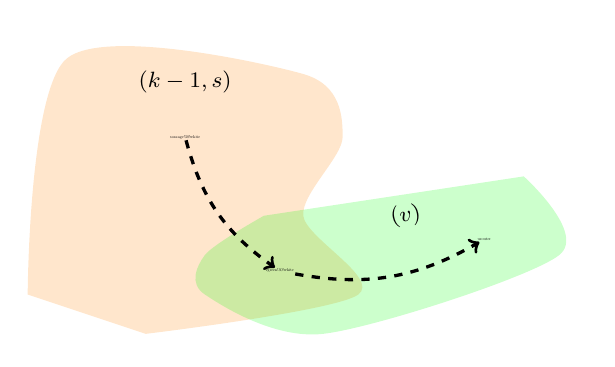
\begin{tikzpicture}
\fill[orange, opacity = 0.2] plot [smooth] coordinates { 
(-1.5, -1) 
(-1, 2) 
(2, 1.8) 
(2.5, 1) 
(2, 0) 
(2.7, -1) 
(0, -1.5)
};

\fill[green, opacity = 0.2, xscale = 1.5] plot [smooth] coordinates { 
(1.5-0.5, 0) 
(1-0.5, -0.5) 
(1-0.5, -1) 
(2-0.5, -1.5)
(4-0.5, -0.5) 
(3.7-0.5, 0.5)
};


\node[scale=0.15] (v) at (0.5, 1) {\router{s}{orange!30!white}};
\node[scale=0.15] (u) at (1.7, -0.7) {\router{v}{green!30!white}};
\node[scale=0.15] (x) at (4.3, -0.3) {\router{u}{router}};

\node at (0.5, 1.7) {\footnotesize $\nreach(k - 1, s)$};
\node[rotate=10] at (3.3, 0) {\footnotesize $\spreach(v)$};

\draw (v) edge[very thick, below, bend right=20, dashed, ->] (u);
\draw (u) edge[very thick, below, bend right=20, dashed, ->] (x);

%\draw (s) edge[very thick, below, bend right=10, dashed, ->] node {$\mathit{sol}(i - 1, y)$} (y);
%\draw (y) edge[very thick, bend right=10, dashed, ->, below] node {$w(y, x)$} (x);
%\draw (s) edge[very thick, bend left=40, dashed, ->, above] node {$\mathit{sol}(i - 1, x)$} (x);
%\draw (s) edge[very thick, bend right=30, dashed, ->] (z);
%\draw (z) edge[very thick, ->, sloped, below] node {$w((z, x))$} (x);
%\draw (s) edge[very thick, bend right=30, dashed, ->, below, sloped] node {$\mathit{sol}(i - 2, r)$} (r);
%\draw (r) edge[very thick, bend right=20, dashed, ->, below, sloped] node {$w(r, z)$} (z);

\end{tikzpicture}
\end{center}
\caption{Illustration of the first part of the recurrence of $\nreach(k, s)$}
\label{fig:nreachC1}
\end{figure}

\begin{figure}
\begin{center}
\begin{tikzpicture}

\fill[orange, opacity = 0.2] plot [smooth] coordinates { 
(-1.5, -1) 
(-1, 2) 
(2, 1.8) 
(2.5, 1) 
(2, 0) 
(2.7, -1) 
(0, -1.5)
};

\def\x{0}
\fill[green, opacity = 0.2, xscale = 2] plot [smooth] coordinates { 
(1.5-0.5+\x, 0) 
(1-0.5+\x, -0.5) 
(1-0.5+\x, -1) 
(2-0.5+\x, -1.5)
(4-0.5+\x, -0.5) 
(3.7-0.5+\x, 0.5)
};


\node[scale=0.15] (v) at (0.5, 1) {\router{s}{orange!30!white}};
\node[scale=0.15] (u) at (1.7, -0.7) {\router{v}{green!30!white}};
\node[scale=0.15] (u1) at (4.3+1, -0.3) {\router{u1}{router}};
\node[scale=0.15] (u2) at (4.3+1, -0.3+1.3) {\router{u2}{router}};

\node[above = 0.1cm of u2] {$u_2 = u$};

\node at (0.5, 1.7) {\footnotesize $\nreach(k - 2, s)$};
\node[rotate=7] at (3.5, -0.2) {\footnotesize $\spreach(v)$};

\draw (v) edge[very thick, below, bend right=20, dashed, ->] (u);
\draw (u) edge[very thick, below, bend right=20, dashed, ->] (u1);
\draw[->, very thick] (u1) -- (u2);

%\draw (s) edge[very thick, below, bend right=10, dashed, ->] node {$\mathit{sol}(i - 1, y)$} (y);
%\draw (y) edge[very thick, bend right=10, dashed, ->, below] node {$w(y, x)$} (x);
%\draw (s) edge[very thick, bend left=40, dashed, ->, above] node {$\mathit{sol}(i - 1, x)$} (x);
%\draw (s) edge[very thick, bend right=30, dashed, ->] (z);
%\draw (z) edge[very thick, ->, sloped, below] node {$w((z, x))$} (x);
%\draw (s) edge[very thick, bend right=30, dashed, ->, below, sloped] node {$\mathit{sol}(i - 2, r)$} (r);
%\draw (r) edge[very thick, bend right=20, dashed, ->, below, sloped] node {$w(r, z)$} (z);

\end{tikzpicture}
\end{center}
\caption{Illustration of the second part of the recurrence of $\nreach(k, s)$}
\label{fig:nreachC2}
\end{figure}

The general intuition for computing the nodes in $\nreach(k, s)$ is provided in 
Figures \ref{fig:nreachC1} and \ref{fig:nreachC2}. Recall that a node $u$ belongs to
$\nreach(k, s)$ if there is a deterministic sr-path from $s$ to $u$ of segment cost at most $k$.
Such a path can have two forms, depending on the type of its last segment. If it is a node segment,
then it is composed by a deterministic sr-path of cost at most $k - 1$ to some node $v$ and then
appended a node segment on $u$ (provided that there is a unique shortest path between $v$ and $u$) as
shown in Figure \ref{fig:nreachC1}. 
Otherwise, it will be made of a deterministic sr-path of cost at most $k - 2$ to some node $v$
and then will be appended an adjacency segment over some edge ending in $u$ as shown in Figure
\ref{fig:nreachC2}. The following theorem formalizes this intuition.

\begin{theorem}
\label{thm:nreach}
Let $G$ be a network, $s \in V(G)$ and an integer $k \geq 3$. It holds that
\begin{align*}
\nreach(1, s) = & \ \{ s \} \\
\nreach(2, s) = & \ \{ v \in V(G) \mid  \sp(s, v) \textrm{ is a path} \} \cup \{ u \mid (s, u) \in E(G) \} \\
\nreach(k, s) = & \ \bigcup_{v \in \nreach(k - 1, s)} \spreach(v) \quad \cup \\ 
& \ \bigcup_{v \in \nreach(k - 2, s)}  \left\{ u_2 \mid (u_1, u_2) \in E(G) \wedge u_1 \in \spreach(v) \right\}
\end{align*}
\end{theorem}

\begin{proof}
For $k = 1$ the only sr-path of cost $1$ starting from $s$ is $\langle s \rangle$. Thus $\nreach(1, s) = \{ s \}$.
For $k = 2$, a sr-path of cost $2$ starting at $s$ has either the form $\langle s, v \rangle$ where
$v \in V(G)$ or $\langle e \rangle$ where $e \in \oute(s)$. In the first case, since we need the sr-path to
be deterministic, only nodes $v \in V(G)$ such that $\sp(s, v)$ is a path yield a deterministic sr-path. In the second case,
a path of the form $\langle e \rangle$ is always deterministic so each such edge yields a valid path.

Let $k \geq 3$. 

$(\subseteq)$ Suppose that $u \in \nreach(k, s)$. Then there exists a deterministic sr-path 
$\sr{p} = \langle x_1, \ldots, x_l \rangle$ from $s$ to $u$ of segment cost at most $k$.
%Since $\sr{p}$ is deterministic, so are $\langle x_1, \ldots, x_{l - 1} \rangle$ and
%$\langle x^2_{l - 1}, x_l \rangle$.

\emph{Case 1:} $x_l = u$ is a node segment.
Then $\langle x_1, \ldots, x_{l - 1} \rangle$ is a deterministic
sr-path from $s$ to $x^2_{l - 1}$ with segment cost at most $k - 1$. Hence $x^2_{l - 1} \in \nreach(k - 1, s)$. By determinism of $\sr{p}$, there is a unique shortest path
between $x^2_{l - 1}$ and $x^1_l = x_l$. Therefore, $u = x_l \in \spreach(x^2_{l - 1})$. Thus letting $v = x^2_{l - 1}$, we have that
$v \in \nreach(k - 1, s)$ and $u \in \spreach(v)$ so
$$
u \in \bigcup_{v \in \nreach(k - 1, s)} \spreach(v).
$$

\emph{Case 2:} $x_l$ is an adjacency segment.
Write $x_l = (u_1, u_2)$. Then $\langle x_1, \ldots, x_{l - 1} \rangle$ is a deterministic sr-path 
from $s$ to $x^2_{l - 1}$ with segment cost at most $k - 2$ and by determinism, 
$u_1 = x^1_l \in \spreach(x^2_{l - 1})$. Thus letting $v = x^2_{l - 1}$,
we have that $v \in \nreach(k - 2, s)$ and $u_1 \in \spreach(v)$ proving that
$$
u = u_2 \in \bigcup_{v \in \nreach(k - 2, s)}  \left\{ u_2 \mid (u_1, u_2) \in E(G) \wedge u_1 \in \spreach(v) \right\}
$$

$(\supseteq)$
Let $u \in \bigcup_{v \in \nreach(k - 1, s)} \spreach(v)$. Then there exists $v \in \nreach(k - 1, s)$
such that $u \in \spreach(v)$. Let $\sr{p} = \langle x_1, \ldots, x_l \rangle$ be a deterministic sr-path from $s$ to $v$ with
$\cost(\sr{p}) \leq k - 1$. Since $u \in \spreach(v)$, there is a unique shortest path from $v$ to $u$ so the
sr-path $\langle x_1, \ldots, x_l, u \rangle$ is a deterministic sr-path from $s$ to $u$ with segment cost
at most $k - 1 + 1 = k$. Thus $u \in \nreach(k, s)$.

Let $u \in \bigcup_{v \in \nreach(k - 2, s)}  \left\{ u_2 \mid (u_1, u_2) \in E(G) \wedge u_1 \in \spreach(v) \right\}$. 
Then there exists $v \in \nreach(k - 2, s)$ and $(u_1, u_2) \in E(G)$ such that $u_1 \in \spreach(v)$ and
$u_2 = u$. Let $\sr{p} = \langle x_1, \ldots, x_l \rangle$ be a sr-path from $s$ to $v$ with segment
cost at most $k - 2$. Then $\langle x_1, \ldots, x_l, (u_1, u_2) \rangle$ is a deterministic sr-path from $s$ to $u$ with
segment cost at most $k - 2 + 2 = k$ from $s$ to $u$ so $u \in \nreach(k, v)$.
\end{proof}

Using Theorem \ref{thm:nreach} we can easily write down an algorithm for computing $\nreach(k, s)$ for all $k, s$.
Algorithm \ref{algo:nreach} is designed so that at the end of its execution it computes a
$\nreach(k, s)$ as a matrix for all relevant values of $k$ and $s$. It will go on until we reach a value
$k'$ such that $\nreach(k', s) = V(G)$ for all $s \in V(G)$. For $k > k'$ we know that $\nreach(k, s) = \nreach(k', s)$
so there is no point in computing it. Its correctness is provided by Theorem \ref{thm:nreach} since it quite literally
implements the recurrences provided by the theorem. It uses Algorithm \ref{algo:spreach} to compute the deterministic
shortest path reach defined in Definition \ref{def:spreach}. This algorithms uses Dijkstra's algorithm to compute the shortest path
DAG rooted at the given node $s$ and the performs a BFS to compute the set of nodes in this DAG that are reachable 
from $s$ via a unique shortest path. On line \ref{algo:spreach_if} of Algorithm \ref{algo:spreach} we ensure that only nodes with unique shortest paths from $s$ are visited by
only adding new nodes to the queue when their in-degree in the shortest path DAG is equal to $1$, as those nodes are the only
ones for which unique shortest paths exist.

\begin{algorithm}[t]
\small
\caption{$\textsf{compute-reach}\left( g \right)$}
\begin{algorithmic}[1]
\STATE $reach \gets \textsf{Matrix}(3, |V(G)|, \textsf{Set}())$
\FOR{$v \in g.\textsf{V}()$}
  \STATE $reach(1, v).\textsf{add}(v)$
\ENDFOR
\STATE $spreach \gets \textsf{Array}(|V(G)|)$
\FOR{$v \in g.\textsf{V}()$}
  \STATE $spreach(v) \gets \textsf{compute-sp-reach}(g, v)$
  \STATE $reach(2, v).\textsf{or}(spreach(v))$
  \FOR{$(u_1, u_2) \in \delta^+(g, s)$}
    \STATE $reach(2, v).\textsf{add}(u_2)$
  \ENDFOR
\ENDFOR
\STATE $k \gets 3$
\WHILE{ $\exists s \in V(g) \ reach(k - 1, v) \neq V(G)$ }
  \FOR{$s \in V(G)$}
    \IF{$reach(k - 1, s) = V(G)$}
      \STATE $reach(k, s) = V(G)$
    \ELSE
      \STATE $reach.\textsf{addRow}(\textsf{Set}())$
      \FOR{$v \in reach(k - 1, s)$}
        \STATE $reach(s, k).\textsf{or}(spreach(v))$
      \ENDFOR
      \FOR{$v \in reach(k - 2, s)$}
        \FOR{$(u_1, u_2) \in E(g)$ \textbf{such that} $u_1 \in spreach(v)$}
	  \STATE $reach(s, k).\textsf{add}(u_2)$
        \ENDFOR
      \ENDFOR
    \ENDIF
  \ENDFOR
\ENDWHILE
\RETURN $nreach$
\end{algorithmic}
\label{algo:nreach}
\end{algorithm}

\begin{algorithm}[t]
\small
\caption{$\textsf{compute-sp-reach}\left( g, s \right)$}
\begin{algorithmic}[1]
\STATE $dag \gets \textsf{dijkstra-dag(v)}$
\STATE $visited \gets \textsf{Set}()$
\STATE $Q \gets \textsf{Queue}()$
\STATE $Q.\textsf{add}(s)$
\WHILE{$|Q| > 0$}
  \STATE $cur \gets Q.\textsf{poll}()$
  \FOR{$(u_1, u_2) \in \delta^+(dag, cur)$ \textbf{such that} $u_2 \notin visited$ \textbf{and} $|\delta^-(dag, u_2)| = 1$} \label{algo:spreach_if}
    \STATE $Q.\textsf{add}(u_2)$
    \STATE $visited.\textsf{add}(u_2)$
  \ENDFOR
\ENDWHILE
\RETURN $visited$
\end{algorithmic}
\label{algo:spreach}
\end{algorithm}

\begin{lemma}
\label{lemma:reachminseg}
Let $G$ be a network, $u, v \in V(G)$ and $k$ a non-negative integer. If $u \notin \nreach(k, v)$ then the minimum segment cost sr-path
between $v$ and $u$ has segment cost at least $k + 1$.
\end{lemma}

\begin{proof}
By definition, if there exists a sr-path $\sr{p}$ between $v$ and $u$ such that $\cost(\sr{p}) \leq k$ then
$u  \in \nreach(k, v)$. Therefore, if $u \notin \nreach(k, v)$, any sr-path between $v$ and $u$ must have a segment cost larger than $k$.
\end{proof}

\begin{corollary}
\label{cor:reachminseg}
Let $G$ be a network, $u, v \in V(G)$ and $k$ a non-negative integer. If $u \notin \nreach(k, v)$ then
any path on $G$ from $v$ to $u$ requires at least $k$ segments in its minimal segmentation.
\end{corollary}

\begin{proof}
Immediate from Lemma \ref{lemma:reachminseg}.
\end{proof}

The two following measures are interesting to evaluate how suitable a topology is for segment routing.

\begin{definition}
We denote the maximum $k$ for which there exists $v \in V(G)$ such that $\nreach(k, n) \neq V(G)$ as $\kM(G)$ and
the minimum $k$ such that there exists $v \in V(G)$ such that $\nreach(k, v) = V(G)$ as $\km(G)$.
\end{definition}

The value of $\kM(G)$ describes the worst case reachability of any node in the network. By Corollary \ref{cor:reachminseg}, it means that there exists
a pair of nodes $u, v$ such that any path from $u$ to $v$ requires at last $\kM(G)$ segments in its minimal
segmentation. Therefore, in a network where routers do not support $\kM(G)$ segments, any solution to a problem
with a path from $u$ to $v$ cannot be implemented on that network. Also, $\kM(G) + 1$ indicates the minimum number of segments that
routers need to suppose in order to be able to implement a multi-cast tree rooted at any node (a spanning tree rooted at that node).
On the other hand, $\km(G)$ gives the maximum value for which some
node $v$ is able to reach every other node. For a network, this means that there exists a multi-cast tree rooted at 
$v$ such that any root to leaf path is segmentable with at most $k$ segments.

We computed these values for every topology in our dataset. Figure \ref{fig:kminkmax} shows the percentage of topologies for each value of 
$\kM(G)$ and $\km(G)$.

\begin{figure}
\begin{center}
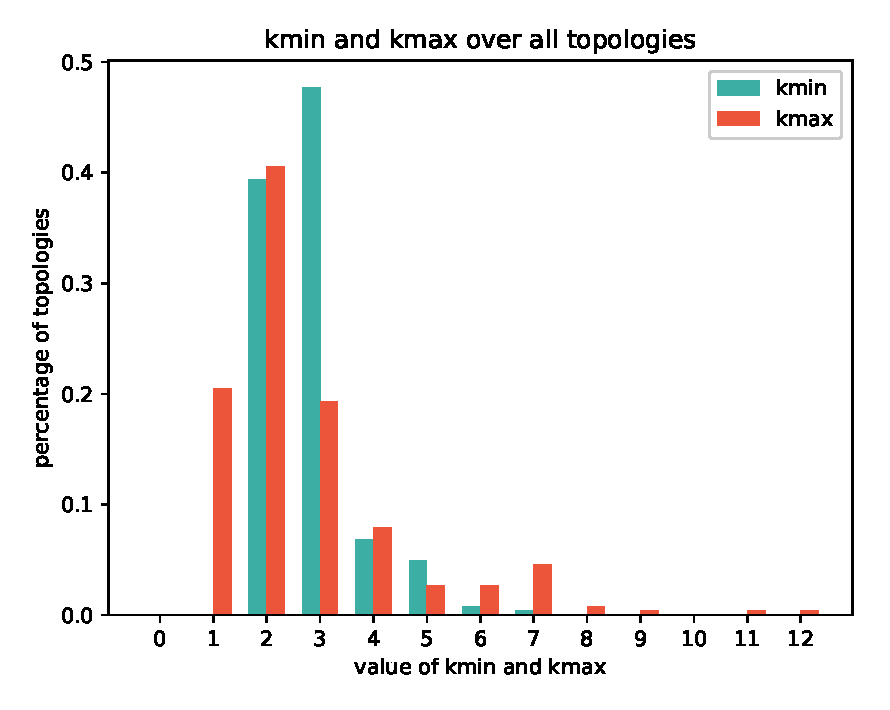
\includegraphics[width=.85\columnwidth]{./Network-lib/data/plot/kminkmax.eps}
\end{center}
\caption{Percentage of topologies for each given value of $\km(G)$ and $\kM(G)$.}
\label{fig:kminkmax}
\end{figure}

In the figure we observe that for $20\%$ of the instances, $\kM(G) = 1$. This means that with two segments, every node
can reach every other node with a deterministic sr-path. In other words, $20\%$ of the topologies do not contain ECMP which matches our analysis
of the topologies in Chapter \ref{chapter:dataset}. We also observe that in the worst case we need up to $12$ segments
to connect some pairs of nodes with a determinism sr-path. This value exceeds the capacity of most commercial routers but very few topologies
are in this case. For $90\%$ of the topologies, with at most $5$ segments any pair of routers can be connected with a deterministic sr-path.

We observe that for $87\%$ of the topologies, there exists some router on the network which is able to reach each other router with a deterministic
sr-path of segment cost at most $3$. We also see that we never need a sr-path path with segment cost larger than $7$ in order to find a root for a multi-cast tree implementable with segment routing.

These results are quite positive and indicate that path based solutions to networking optimization problems are likely to be
implementable with segment routing. This result is not a definitive answer as the measure that we would really like to compute in order to be able to answer these
questions is the maximum number of segments needed to represent any simple path in the original network. This would give an
upper bound on the number of segments required for implementing any path based solution with segment routing on each topology. 
Unfortunately computing this value is \NPhard~as we shown next.

%In this section we are going to study the problem of estimating the minimum number of
%segments required on a given network. We will start by showing that computing the 
%maximum number of segments required to minimaly segment any simple path in the network
%is \NPhard.

\begin{problem}{Maximum segmentation path}
\label{prob:max-seg}
Given a network $G$ compute the maximum value of $\cost(\mseg(p))$ such that $p$ is a simple path in $G$.
\end{problem}

In order to prove that Problem \ref{prob:max-seg} is \NPhard~ we need to defined some related problems first.
The first problem that we consider is the same except that we only focus on paths between two given nodes.

\begin{problem}{Maximum segmentation $s$-$t$ path}
\label{prob:max-seg-st}
Given a network $G$ and $s, t \in V(G)$ find a simple $s$-$t$ path $p$ such that $\cost(\mseg(p))$ is maximum.
\end{problem}


\begin{problem}{Unit weights longest path between nodes}
\label{prob:lpst}
Given a graph $G$ and $s, t \in V(G)$ compute the longest path from $s$ to $t$ in terms of the number of links
in the path.
\end{problem}

\begin{theorem}
Problem \ref{prob:lpst} is \NPhard. 
\end{theorem}

\begin{proof}
This is a known result. A proof can be found, for instance, in Corollary 8.11a from \cite{schrijver-book}.
\end{proof}

\begin{theorem}
\label{thm:max-seg-st-np}
Problem \ref{prob:max-seg-st} is \NPhard. 
\end{theorem}

\begin{proof}
We are going to prove that Problem \ref{prob:max-seg-st} is \NPhard by showing that
if we could solve it in polynomial time, then we could also solve Problem \ref{prob:lpst} in polynomial time.

Let $G, s, t$ be an instance of Problem \ref{prob:lpst}. Build a graph $H$ which is a copy of $G$ to which we add the following. For each
edge $(u, v) \in E(G)$, add a node $uv$ and two edges $(u, uv)$ and $(uv, v)$ both of weight $1$. Figure \ref{fig-np-max-seg}
illustrates this transformation.

\begin{figure}[H]
\begin{center}
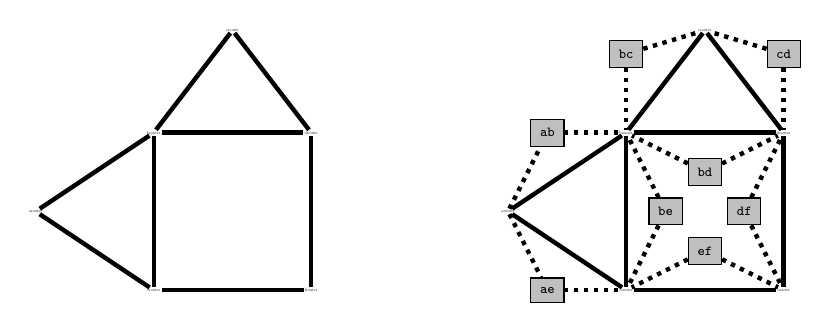
\begin{tikzpicture}
\def\dx{0}
%\node[draw, circle, fill=lightgray] (a) at (\dx + 0, 0) {\tiny \texttt{a}};
%\node[draw, circle, fill=lightgray] (b) at (\dx + 1, 1) {\tiny \texttt{b}};
%\node[draw, circle, fill=lightgray] (c) at (\dx + 2, 2) {\tiny \texttt{c}};
%\node[draw, circle, fill=lightgray] (d) at (\dx + 3, 1) {\tiny \texttt{d}};
%\node[draw, circle, fill=lightgray] (e) at (\dx + 1, -1) {\tiny \texttt{e}};
%\node[draw, circle, fill=lightgray] (f) at (\dx + 3, -1) {\tiny \texttt{f}};

\node[scale=0.15] (a) at (\dx + -0.5, 0) {\router{a}{router}};
\node[scale=0.15] (b) at (\dx + 1, 1) {\router{b}{router}};
\node[scale=0.15] (c) at (\dx + 2, 2.3) {\router{c}{router}};
\node[scale=0.15] (d) at (\dx + 3, 1) {\router{d}{router}};
\node[scale=0.15] (e) at (\dx + 1, -1) {\router{e}{router}};
\node[scale=0.15] (f) at (\dx + 3, -1) {\router{f}{router}};


\draw[ultra thick] (a) -- (b);
\draw[ultra thick] (a) -- (e);
\draw[ultra thick] (b) -- (e);
\draw[ultra thick] (b) -- (c);
\draw[ultra thick] (c) -- (d);
\draw[ultra thick] (b) -- (d);
\draw[ultra thick] (b) -- (e);
\draw[ultra thick] (f) -- (d);
\draw[ultra thick] (f) -- (e);

\def\dx{6}
%\node[draw, circle, fill=lightgray] (a) at (\dx + 0, 0) {\tiny \texttt{a}};
%\node[draw, circle, fill=lightgray] (b) at (\dx + 1, 1) {\tiny \texttt{b}};
%\node[draw, circle, fill=lightgray] (c) at (\dx + 2, 2) {\tiny \texttt{c}};
%\node[draw, circle, fill=lightgray] (d) at (\dx + 3, 1) {\tiny \texttt{d}};
%\node[draw, circle, fill=lightgray] (e) at (\dx + 1, -1) {\tiny \texttt{e}};
%\node[draw, circle, fill=lightgray] (f) at (\dx + 3, -1) {\tiny \texttt{f}};


\node[scale=0.15] (a) at (\dx + -0.5, 0) {\router{a}{router}};
\node[scale=0.15] (b) at (\dx + 1, 1) {\router{b}{router}};
\node[scale=0.15] (c) at (\dx + 2, 2.3) {\router{c}{router}};
\node[scale=0.15] (d) at (\dx + 3, 1) {\router{d}{router}};
\node[scale=0.15] (e) at (\dx + 1, -1) {\router{e}{router}};
\node[scale=0.15] (f) at (\dx + 3, -1) {\router{f}{router}};

\draw[ultra thick] (a) -- (b);
\draw[ultra thick] (a) -- (e);
\draw[ultra thick] (b) -- (e);
\draw[ultra thick] (b) -- (c);
\draw[ultra thick] (c) -- (d);
\draw[ultra thick] (b) -- (d);
\draw[ultra thick] (b) -- (e);
\draw[ultra thick] (f) -- (d);
\draw[ultra thick] (f) -- (e);

\node[draw, fill=lightgray] (ab) at (\dx + 0, 1) {\tiny \texttt{ab}};
\draw[ultra thick, dotted] (a) edge[above, sloped] (ab);
\draw[ultra thick, dotted] (b) edge[above, sloped] (ab);

\node[draw, fill=lightgray] (ae) at (\dx + 0, -1) {\tiny \texttt{ae}};
\draw[ultra thick, dotted] (a) edge[below, sloped] (ae);
\draw[ultra thick, dotted] (e) edge[below, sloped] (ae);

\node[draw, fill=lightgray] (bc) at (\dx + 1, 2) {\tiny \texttt{bc}};
\draw[ultra thick, dotted] (bc) edge[below, sloped] (b);
\draw[ultra thick, dotted] (bc) edge[below, sloped] (c);

\node[draw, fill=lightgray] (cd) at (\dx + 3, 2) {\tiny \texttt{cd}};
\draw[ultra thick, dotted] (cd) edge[below, sloped] (c);
\draw[ultra thick, dotted] (cd) edge[below, sloped] (d);

\node[draw, fill=lightgray] (bd) at (\dx + 2, 0.5) {\tiny \texttt{bd}};
\draw[ultra thick, dotted] (bd) edge[sloped] (b);
\draw[ultra thick, dotted] (bd) edge[sloped] (d);

\node[draw, fill=lightgray] (be) at (\dx + 1.5, 0) {\tiny \texttt{be}};
\draw[ultra thick, dotted] (be) edge[sloped] (b);
\draw[ultra thick, dotted] (be) edge[sloped] (e);

\node[draw, fill=lightgray] (ef) at (\dx + 2, -0.5) {\tiny \texttt{ef}};
\draw[ultra thick, dotted] (ef) edge[sloped] (e);
\draw[ultra thick, dotted] (ef) edge[sloped] (f);

\node[draw, fill=lightgray] (df) at (\dx + 2.5, 0) {\tiny \texttt{df}};
\draw[ultra thick, dotted] (df) edge[sloped] (d);
\draw[ultra thick, dotted] (df) edge[sloped] (f);

\end{tikzpicture}
\end{center}
\caption{Example of the transformation. Solid edges have weight $2$ whereas dotted edges have weight $2$.}
\label{fig-np-max-seg}
\end{figure}

Let $p$ be a path on $H$ from $s$ to $t$ such that $\cost(\mseg(p))$ is maximum. We start by proving that $p$
does not cross any of the new nodes, that is, only crosses nodes in $V(G) \cap V(H)$. Suppose that $p$ visits the node
sequence $(v_1, \ldots, v_l)$ and let $i$ be the smallest index such that $v_i \notin V(G)$. Since $p$ is a path from
$s$ to $t$ and $s, t \in V(G)$ we have that $1 < i < l$. Thus we can write $v_i = v_{i-1}v_{i+1}$ and 
$p = (v_1, \ldots, v_{i - 1}, v_i, v_{i + 1}, \ldots, v_l) = (v_1, \ldots, v_{i - 1}, v_{i - 1} v_{i+1}, v_{i +1} \ldots, v_l)$.
We need to consider three cases.

\emph{Case 1:} $v_{i + 2} \in V(G)$. In this case path $p$ has the form:

\begin{center}

\begin{tikzpicture}[scale=0.8]
\node[scale=0.15] (v1) at (0, 0) {\router{$v_1$}{router}};
\node (dots) at (2, 0) {$\ldots$};
\node[scale=0.15] (vi-1) at (4, 0) {\router{$v_{i - 1}$}{router}};
\node[draw, fill=lightgray] (vi) at (6, 0) {\footnotesize $v_{i-1}v_{i+1}$};
\node[scale=0.15] (vi+1) at (8, 0) {\router{$v_{i + 1}$}{router}};
\node[scale=0.15] (vi+2) at (10, 0) {\router{$v_{i + 2}$}{router}};
\node (dots2) at (11, 0) {$\ldots$};

\draw (v1) edge[line width=2, ->] (dots);
\draw (dots) edge[line width=2, ->] (vi-1);
\draw (vi-1) edge[line width=2, dotted, ->] (vi);
\draw (vi) edge[line width=2, dotted, ->] (vi+1);
\draw (vi+1) edge[line width=2, ->] (vi+2);
\end{tikzpicture}
\end{center}

By construction, every link of $G$ that is traversed requires an adjacency segment
in its minimal segmentation (because of ECMP). 
Therefore, the minimal segmentation of this path is 
$$
\langle (v_1, v_2), (v_2, v_3), \ldots, (v_{i - 2}, v_{i - 1}), xy, (v_{i + 1}, v_{i + 2}), \ldots \rangle.
$$
On the other hand, if we remove element $xy$ from the path, we obtain a simple path $p'$ with the same minimal segmentation
except that $xy$ is replaced by the adjacency segment $(x, y)$ giving
$$
\langle (v_1, v_2), (v_2, v_3), \ldots, (v_{i - 2}, x), (x, y), (y, v_{i + 2}), \ldots \rangle.
$$
This segmentation costs one more than the segmentation of $p$. Since $p'$ is also a path from $s$ to $t$, this 
contradicts the fact that $p$ is a path from $s$ to $t$ that maximizes $\cost(\mseg(p))$.

\emph{Case 2:} $v_{i + 2} \notin V(G)$. In this case, $p$ has the following form:

\begin{center}
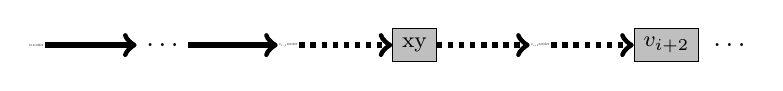
\begin{tikzpicture}[scale=0.8]
\node[scale=0.15] (v1) at (0, 0) {\router{$v_1$}{router}};
\node (dots) at (2, 0) {$\ldots$};
\node[scale=0.15] (vi-1) at (4, 0) {\router{$v_{i - 1}$}{router}};
\node[draw, fill=lightgray] (vi) at (6, 0) {\footnotesize xy};
\node[scale=0.15] (vi+1) at (8, 0) {\router{$v_{i + 1}$}{router}};
\node[draw, fill=lightgray] (vi+2) at (10, 0) {\footnotesize $v_{i + 2}$};
\node (dots2) at (11, 0) {$\ldots$};

\draw (v1) edge[line width=2, ->] (dots);
\draw (dots) edge[line width=2, ->] (vi-1);
\draw (vi-1) edge[line width=2, dotted, ->] (vi);
\draw (vi) edge[line width=2, dotted, ->] (vi+1);
\draw (vi+1) edge[line width=2, dotted, ->] (vi+2);
\end{tikzpicture}
\end{center}

The minimal segmentation of $p$ will be
$$
\langle (v_1, v_2), (v_2, v_3), \ldots, (v_{i - 2}, x), xy, v_{i + 2}, \ldots \rangle.
$$
As before, if we remove $xy$ from $p$ we obtain a simple path $p'$ from $s$ to $t$
with minimal segmentation equal to
$$
\langle (v_1, v_2), (v_2, v_3), \ldots, (v_{i - 2}, x), (x, y), v_{i + 2}, \ldots \rangle.
$$
This segmentation costs one more than the minimal segmentation of $p$ so as above, we conclude
that $p$ does not minimize $\cost(\mseg(p))$.

These two cases cover all possibilities so we conclude that the path $p$ on $H$ that maximizes
$\cost(\mseg(p))$ has all of its nodes in $V(G)$. Therefore, this is also a path in $G$.
Furthermore, because of ECMP, that the minimal segmentation of $p$ will contain
all of its edges as adjacency segments. Hence $\cost(\mseg(p)) = 2 |E(p)|$ so it follows that
if can find a path on $H$ that maximizes $\cost(\mseg(p))$ we can find a path on $G$ that maximizes
$E(p)$ which completes the proof.
% 
% 
% \newpage
% 
% Let $p = (v_1, v_2, \ldots, v_k)$ be a simple path in $G$. By theorem \todo{adjacency segment theorem}, each edge of path $p$
% requires an adjacency segment. Therefore, $\mseg(p) = \langle (v_1, v_2), (v_2, v_3), \ldots, (v_{k - 1}, v_k) \rangle$.
% 
% Let $p = (u_1, u_2, \ldots, u_k)$ be a path in $H$ such that $\cost(\mseg(p))$ is maximum. We are going to prove that
% there exists a path $q$ containing only nodes in $V(G)$ with the same segmentation cost.
% 
% 
% If $u_i \in V(G)$ for each $i = 1, \ldots, k$ then there is noting to prove. Othersiwe, let $i$ by the minimum index
% such that $u_i \notin V(G)$. Write $u_i = xy$ where $x, y \in V(G)$.
% 
% Then $p$ has the form $(u_1, \ldots, u_{i - 1}, u_i, u_{i + 1} \ldots) = (u_1, \ldots, x, xy, y, \ldots)$.
% The minimal segmentation of $p$ must has the form $\langle (u_1, u_2), (u_2, u_3), \ldots, (u_{i - 1}, x), \ldots, \rangle$
% 
% The minimal segmentation $\sr{p}$ of $p$ on $H$ is easy to characterize. 
% It will contain all special nodes $u_i \notin V(G)$ as node segments
% together with all edges $(u_i, u_{i + 1}) \in E(G)$ as adjacency segemnts (in their order of appearence). Finally,
% if $(u_1, u_2) \notin E(G)$ then $u_1$ will apprear as the first node and if $(u_{k - 1}, u_k) \notin E(G)$, then $u_k$
% will appear as the last node.
% 
% Therefore, if we remove the first special node $u_i \notin V(G)$ from $p$
% 
% \todo{STEPS:
% \begin{itemize}
%  \item Prove the structure of minimal segmentations on $H$
%  \item Prove that we can replace the first special node $ab$ by $b$. 
%  We need to make sure that the segment cost is not reduced and that we still have a simple path.
%  \item With this we show that there exists a solution of the problem that is a path in $G$.
%  \item We show that any path in $G$ maps to a path in $H$ with double segment cost.
%  \item We conclude that if there was a longer path in $G$ then we would have a longer segmentation
% \end{itemize}
% }
% 
% For instance, path $(a, ab, b, bc, c, d)$ has minimal segmentation $\langle a, ab, bc, (c, d) \rangle$.

\end{proof}

\begin{corollary}
Problem \ref{prob:max-seg} is \NPhard. 
\end{corollary}

\begin{proof}
Let $G, s, t$ be an instance of Problem \ref{prob:max-seg-st}. 
%We will build an instance $G'$ of Problem \ref{prob:max-seg}
%whose answer is the optimal solution of Problem \ref{prob:max-seg-st} plus some constant $C$. 
Let $m = E(G)$. We build a graph by adding a path $(x_1, \ldots, x_m, s)$ connecting to $s$ whose minimal segmentation 
has segment cost $2 m$ and a path $(t, y_1, \ldots, y_m)$ going out of $t$ whose minimal segmentation also has segment cost
$2 m$. This is achieved by adding also nodes $x'_1, \ldots, x'_m$ and $y'_1, \ldots, y'_m$ and edges $(x_i, x'_i)$ and
$(x'_i, x_{i + 1})$ of cost $1$ to ensure that adjacency segments are required to segment the two paths
mentioned above. Figure \ref{fig:np-transform2} illustrates this. Dashed edges represent edges of cost $1$
and solid edges represent edge of cost $2$.

\begin{figure}[H]
\begin{center}
\begin{tikzpicture}[scale=0.8]
\draw[ultra thick, lightgray, fill=lightgray!50!white] (0, 0) circle (2);
\node[scale=0.15] (s) at (-0.75, -0.75) {\router{$s$}{router}};
\node[scale=0.15] (t) at (0.75, 0.75) {\router{$t$}{router}};
\node[] (g) at (-1, 1) {$G$};

\node (gg) at (-5, 2) {$G'$};

\node[scale=0.15] (xm) at (-2.5, -0.75) {\router{$x_m$}{router}};
\node[scale=0.15] (xxm) at (-2.5, -3) {\router{$x'_m$}{router}};
\node[scale=0.15] (xm-1) at (-4.5, -0.75) {\router{$x_{m - 1}$}{router}};
\node[scale=0.15] (xxm-1) at (-4.5, -3) {\router{$x'_{m-1}$}{router}};
\node at (-5.5, -0.75) {$\ldots$};
\node[scale=0.15] (x1) at (-6.5, -0.75) {\router{$x_{1}$}{router}};
\node[scale=0.15] (xx1) at (-6.5, -3) {\router{$x'_{1}$}{router}};

\draw (xm) edge[line width=2, dotted, ->] (xxm);
\draw (xxm) edge[line width=2, dotted, ->] (s);
\draw (xm) edge[line width=2, ->] (s);

\draw (xm-1) edge[line width=2, dotted, ->] (xxm-1);
\draw (xxm-1) edge[line width=2, dotted, ->] (xm);
\draw (xm-1) edge[line width=2, ->] (xm);
\draw (x1) edge[line width=2, ->, dotted] (xx1);

\node[scale=0.15] (ym) at (2.5, 0.75) {\router{$y_m$}{router}};
\node[scale=0.15] (yym) at (2.5, 3) {\router{$y'_m$}{router}};
\node[scale=0.15] (ym-1) at (4.5, 0.75) {\router{$y_{m - 1}$}{router}};
\node[scale=0.15] (yym-1) at (4.5, 3) {\router{$y'_{m-1}$}{router}};
\node at (5.5, 0.75) {$\ldots$};
\node[scale=0.15] (y1) at (6.5, 0.75) {\router{$y_{1}$}{router}};
\node[scale=0.15] (yy1) at (6.5, 3) {\router{$y'_{1}$}{router}};


\draw (ym) edge[line width=2, dotted, <-] (yym);
\draw (yym) edge[line width=2, dotted, <-] (t);
\draw (ym) edge[line width=2, <-] (t);

\draw (ym-1) edge[line width=2, dotted, <-] (yym-1);
\draw (yym-1) edge[line width=2, dotted, <-] (ym);
\draw (ym-1) edge[line width=2, <-] (ym);
\draw (y1) edge[line width=2, <-, dotted] (yy1);

\draw[cyan, line width=2, ->] plot [smooth] coordinates { ($(x1)+(0,0.5)$) ($(xm-1)+(0,0.5)$) ($(xm)+(0,0.5)$)  ($(s)+(0,0.5)$) ($(s)+(0.5,0.5)$) ($(t)+(0,-0.5)$) ($(ym)+(0,-0.5)$) ($(ym-1)+(0,-0.5)$) ($(y1)+(0,-0.5)$)};



\end{tikzpicture}
\end{center}
\caption{Example of the transformation.}
\label{fig:np-transform2}
\end{figure}

By lemma \ref{lemma:edgeseg}, the maximum cost of a minimal segmentation in $G$ is at most $2 m$. Therefore,
the maximum cost of a minimal segmentation of a path in $G'$ must be a path from $x_1$ to $y_1$ since just this part
of the path will have segment cost at least $4m$. Since the path from $x_1$ passes by $s$, to each
$y_1$ we need to pass by $t$, we will achieve the maximum segment cost by connecting $s$ and $t$ by path with maximum 
segmentation cost. Thus the solution to Problem \ref{prob:max-seg} on $G'$ is a path of cost $x + 4m$ where $x$ is the cost of
the solution to problem \ref{prob:max-seg-st} on input $G, s, t$. We conclude that if we could solve Problem \ref{prob:max-seg}
in polynomial time then we could also solve Problem \ref{prob:max-seg-st} in polynomial time. Therefore, by Theorem \ref{thm:max-seg-st-np},
we conclude that \ref{prob:max-seg} is \NPhard.


\end{proof}



% ------------------------------------------------------------
% 
% \todo{this needs to be fixed, it still uses $\ereach(2, v)$ assuming that it mean unique shortest path}
% 
% \begin{theorem}
% \label{thm:ereach}
% Let $G$ be a network, $s \in V(G)$ and an integer $k \geq 3$. It holds that
% \begin{align*}
% \ereach(1, s) = & \ \emptyset \\
% \ereach(2, s) = & \ \{ e \in E(G) \mid \sp(s, v) \textrm{ is a path with last edge $e$} \} \quad \cup \\
%                 & \ \{ (s, u) \mid (s, u) \in E(G) \} \\
% \ereach(k, s) = & \ \bigcup_{v \in \nreach(k - 1, s)} \ereach(2, v) \quad \cup \\ 
% & \ \bigcup_{v \in \nreach(k - 2, s)}  \left\{ (u_1, u_2) \mid (u_1, u_2) \in E(G) \wedge u_1 \in \nreach(2, v) \right\}
% \end{align*}
% \end{theorem}
% 
% \begin{proof}
% For $k = 1$ the only sr-path of cost $1$ starting from $s$ is $\langle s \rangle$ and it contains no edges. Thus $\nreach(1, s) = \emptyset$.
% For $k = 2$, a sr-path of cost $2$ starting at $s$ has either the form $\langle s, v \rangle$ where
% $v \in V(G)$ or $\langle (s, v) \rangle$ where $(s, v) \in E(G)$. Thus, for each $v$ such that $\sp(s, v)$ is a path,
% the last edge will belong to $\ereach(2, s)$. Also, every edge of the form $(s, v)$ will belong to $\ereach(2, s)$
% 
% Let $k \geq 3$.
% 
% $(\subseteq)$ Let $e \in \ereach(k, v)$. Then there exists a deterministic sr-path 
% $\sr{p} = \langle x_1, \ldots, x_{l - 1}, x_l \rangle$  of segment cost at most $k$ such that
% either $x_l = e$ or $x_l$ is a node
% segment and $e$ is the last edge of the unique shortest path between $x^2_{l - 1}$
% and $x_{l}$. Let $\sr{q} = \langle x_1, \ldots x_{l - 1} \rangle$ and $v = x^2_{l - 1}$.
% 
% \emph{Case 1:} $x_l = e = (u_1, u_2)$. Let 
% Since $\cost(\sr{p}) \leq k$, we know that
% $\cost(\sr{q}) \leq k - 2$. Thus $v = x^2_{l - 1} \in \nreach(k - 2, s)$. 
% Since $\sr{p}$ is deterministic, 
% there must be a unique shortest path
% between $x^2_{l - 1} = v$ to $x^1_l = u_1$. Therefore, $u_1 \in \nreach(2, v)$ so
% $$
% e \in \bigcup_{v \in \nreach(k - 2, s)}  \left\{ (u_1, u_2) \mid (u_1, u_2) \in E(G) \wedge u_1 \in \nreach(2, v) \right\}.
% $$
% 
% \emph{Case 2:} $x_l$ is a node segment and $e$ is the last edge of the unique
% shortest path between $x^2_{l - 1}$ and $x_l$. Then $\cost(\sr{q}) \leq k - 1$
% so that $v \in \nreach(s, k - 1)$. Since $e$ is the last edge of the unique
% shortest path between $v = x^2_{l - 1}$ and $x_l$ we have that $e \in \ereach(2, v)$.
% Thus
% $$
% e \in \bigcup_{v \in \nreach(k - 1, s)} \ereach(2, v).
% $$
% 
% $(\supseteq)$ Let $e \in \bigcup_{v \in \nreach(k - 1, s)} \ereach(v, 2)$. Then
% there exists $v \in \nreach(k - 1, s)$ such that $e \in \ereach(v, 2)$. By definition,
% this means that there exists a deterministic sr-path $\sr{p} = \langle x_1, \ldots, x_l \rangle$
% from $s$ to $v$ with $\cost(\sr{p}) \leq k - 1$ and a unique shortest path from $v$ to $u$
% such that $e$ is the last edge of that path. Thus, $\langle x_1, \ldots, x_l, u \rangle$ is a deterministic
% sr-path from $s$ to $u$ of cost at most $k - 1 + 1 = k$ with last edge $e$. We conclude that
% $e \in \ereach(s, k)$.
% 
% Let $(u_1, u_2) \in \bigcup_{v \in \nreach(k - 2, s)}  \left\{ (u_1, u_2) \mid (u_1, u_2) \in E(G) \wedge u_1 \in \nreach(2, v) \right\}$.
% Then there exists $v \in \nreach(k - 2, s)$ such that $u_1 \in \nreach(2, v)$. 
% By definition, this means that we have a deterministic sr-path $\sr{p} = \langle x_1, \ldots, x_l \rangle$ from $s$ to $v$ with segment cost at most $k - 2$ and
% a unique shortest path from $v$ to $u_1$. Therefore $\langle x_1, \ldots, x_l, (u_1, u_2) \rangle$ is a deterministic sr-path
% from $s$ to $u_2$ of segment cost at most $k - 2 + 2 = k$ with last element being an adjacency segment
% on $(u_1, u_2)$. Hence, $(u_1, u_2) \in \ereach(k, s)$.
% \end{proof}


% \begin{proposition}
% Let $G$ be a network, $s \in V(G)$. Then for $k \geq 2$,
% \begin{align*}
% \nreach(0, s) = & \left\{ s \right\} \\
% \nreach(1, s) = & \left\{ V(\sp(s, v)) \mid \textrm{$v \in V(G)$ and $\sp(s, v)$ is a path} \right\} \\
% \nreach(k, s) = & \bigcup_{v \in \nreach(k - 1, s)} \nreach(1, v) \quad \cup \\
%                 & \left\{ u_2 \mid (u_1, u_2) \in E(G) \wedge \exists u \in \nreach(k - 2, s) : u_1 \in \nreach(1, u) \right\}
% \end{align*}
% \end{proposition}
% 
% \begin{proof}
% If $k = 0$ then the only sr-path starting at $s$ of segment cost at most $0$ is $\langle s \rangle$. Thus, since $V(\langle s \rangle) = s$, $\nreach(0, s) = \{ s \}$.
% For $k = 1$, the sr-paths starting at $s$ with segments cost at most $1$ are for the form $\langle s, v \rangle$ for $v \in V(G)$. From these, we only consider the ones
% that are deterministic, that is, the ones such that there is a unique shortest path between $s$ and $v$. In other words, the ones such that $\sp(s, v)$ is a path.
% 
% For $k \geq 2$ we will prove the that each set is contained inside the other. 
% 
% $(\subseteq)$ Let $v \in \nreach(k, s)$. Then, by definition, there exists a deterministic sr-path $\sr{p} = \langle x_1, \ldots, x_l \rangle$
% of cost at most $k$ such that $v \in V(\sr{p})$.
% \end{proof}




% \section{SR formalization}
% 
% In this section we propose a mathematical formalization of segment routing. This is a first step
% towards a uniformisation of the mathematical notations used to represent segments routing problems.
% 
% \todo{more blabla}
% 
% The first thing tht we are going to define are the concepts of node and adjacency segments.
% 
% \begin{definition}
% Let $G$ be a network. We define the \emph{segment set} of $G$ as $\seg(G) = V(G) \cup E(G)$.
% Let $x \in \seg(G)$. If $x = (u, v) \in E(G)$ we write $x^- = u$ and $x^+ = v$.
% Otherwise $x = v \in V(G)$ and we write $x^- = x^+ = v$.
% \end{definition}
% 
% Note that even for node segments we define the notations $x^-$ and $x^+$. As we will see shortly,
% it makes it possible to express other concept in a much more elegent maner as it avoids having
% to distinguish between the times of segments that are under consideration.
% 
% Next, we define the concept of segment routing paths, which essentially capture the segment
% stack that will be provided to the ingress node. The main difference between this definition and the
% ingress node is considered to be part of the path whereas in real netwoks it is not added to the SR stack.
% 
% \begin{definition}
% A \emph{segment routing path (sr-path)} is a sequence $\sr{p} = \langle x_1, \ldots, x_k \rangle$ such that each $x_i \in \seg(G)$ and
% for each $i = 2, \ldots k$, $x^+_{i - 1} \rightsquigarrow x^-_i$. We call $k$ the \emph{length} of $\sr{p}$ and write $\len(\sr{p}) = k$.
% 
% We write $\node(\sr{p}) = \{ x_i \mid x_i \in V(G) \}$ and call its elements \emph{node segments} and $\adj(\sr{p}) = \{ x_i \mid x_i \in E(G) \}$
% and call its elements \emph{adjacency segments}.
% 
% Finally, we define the \emph{segment cost} of $\sr{p}$ as $|\node(\sr{p})| + 2 \cdot |\adj(\sr{p})|$. We write it as $\cost(\sr{p})$.
% \end{definition}
% 
% The reason why adjacency segments have a double weight on the segment cost is because they require two entries in the segment
% stack instead of one. The segment cost is a huge constraint for SR as most routers have a very limited SR stack size \todo{ref}.
% 
% As we saw in the introduction, packets forwarded on a sr-path will follow shortest paths between consecutive segments. It can
% happen that more than one shortest path exists between to consecutive segments. This is called Equal-Cost MultiPath (ECMP) in the
% networking literature \todo{ref}. In this case, depending on the underlying
% application, one of two things can happend: (i) the traffic is split in some way among all those paths for load balancing or (ii)
% a single one of those paths is used to forward the traffic and this selection is done using a hash function. \todo{ref?} In the later case,
% the network operators have no way of knowing apriori which of them will be used.
% 
% In any case, we need a  way to describe all the network links that can contribute to the forwarding of packets between
% two consecutive segments. This leads to the definition of forwarding graphs.
% 
% \begin{definition}
% Let $\sr{p} = \langle x_1, \ldots, x_k \rangle$ be a sr-path. We define the \emph{forwarding graph} of $\sr{p}$ by
% $$
% \forw(\sr{p}) = \left( \bigcup_{i = 2}^k \sp(x^+_{i - 1}, x^-_{i}) \right) \cup \bigcup_{x \in \adj(\sr{p})} x.
% $$
% \end{definition}
% 
% The first part of the defintion of forwarding graphs captures all the shortest paths that are used between consecutive segments
% and the second part captures all links represented by adjacency segments. To better illustrate this defintion let's consider a few examples.
% 
% Figure \ref{fig:sr1} shows, in green, $\forw(\langle a, (d, e), i \rangle)$. To see that it matches the definition, we can write
% \begin{align*}
% \forw(\langle a, (d, e), i \rangle) & = \sp(a^+, (d, e)^-) \cup \sp( (d, e)^+, i^-) \cup (d, e) \\
% & = \sp(a, d) \cup \sp(e, i) \cup (d, e) \\
% & = (a, c, d) \cup (e, h, i) \cup (d, e) \\
% & = \{ (a, c), (c, d), (e, h), (h, i), (d, e) \}.
% \end{align*}
% 
% Consider now the sr-path $\sr{p} = \langle a, b, (d, e), i \rangle$ on the same graph as shown in Figure \ref{fig:sr2}. This
% example illustrates two things. First, from $b$ to the origin of $(d, e)$ there are two shortest paths so we see that
% $\forw(\sr{p})$ corresponds to a subgraph of $G$ and not just a path. Second, we see that the forwarding subgraph can
% contain cycles contrary to what our intuition might suggest. To confirm that this is correct we compute $\forw(\sr{p})$
% once more:
% \begin{align*}
% \forw(\langle a, b, (d, e), i \rangle) & = \sp(a^+, b^-) \cup \sp( b^+, (d, e)^-) \cup \sp( (d, e)^+, i^-) \cup (d, e) \\
% & = \sp(a, b) \cup \sp(b, e) \cup \sp(e, i) \cup (d, e) \\
% & = (a, b) \cup (b, c, d) \cup (b, e, d) \cup (e, h) \cup (h, i) \cup (d, e) \\
% & = \{ (a, b) (b, c), (c, d), (b, e), (e, d), (e, h), (h, i), (d, e) \}.
% \end{align*}
% 
% 
% \begin{figure}[H]
% \begin{center}
% \begin{tikzpicture}
% \def\x{0}
% \def\y{0}
% \node[scale=0.15] (a) at (0.5 + \x,  0.5 + \y) {\router{a}{green}};
% \node[scale=0.15] (b) at (0.5 + \x, -1.0 + \y) {\router{b}{green}};
% \node[scale=0.15] (c) at (2.5 + \x,  0.0 + \y) {\router{c}{lightgray}};
% \node[scale=0.15] (d) at (4.5 + \x,  0.0 + \y) {\router{d}{green}};
% \node[scale=0.15] (e) at (4.0 + \x, -2.0 + \y) {\router{e}{green}};
% \node[scale=0.15] (g) at (6.0 + \x,  0.5 + \y) {\router{g}{lightgray}};
% \node[scale=0.15] (i) at (8.0 + \x,  0.0 + \y) {\router{i}{green}};
% \node[scale=0.15] (h) at (7.0 + \x, -1.5 + \y) {\router{h}{lightgray}};
% \node[scale=0.15] (f) at (4.0 + \x, -3.5 + \y) {\router{f}{lightgray}};
% \node[scale=0.15] (j) at (8.0 + \x, -2.5 + \y) {\router{j}{lightgray}};
% \draw[line width=2] (f) edge[above, sloped] node[black,font=\bfseries] {\tiny \texttt{}} (j);
% \draw[line width=2] (h) edge[above, sloped] node[black,font=\bfseries] {\tiny \texttt{}} (j);
% \draw[line width=2] (a) edge[above, sloped] node[black,font=\bfseries] {\tiny \texttt{}} (b);
% \draw[line width=2] (b) edge[above, sloped] node[black,font=\bfseries] {\tiny \texttt{}} (c);
% \draw[line width=2] (e) edge[above, sloped] node[black,font=\bfseries] {\tiny \texttt{}} (c);
% \draw[line width=2] (b) edge[above, sloped] node[black,font=\bfseries] {\tiny \texttt{}} (e);
% \draw[line width=2] (b) edge[above, sloped] node[black,font=\bfseries] {\tiny \texttt{}} (f);
% \draw[line width=2] (e) edge[above, sloped] node[black,font=\bfseries] {\tiny \texttt{}} (f);
% \draw[line width=2] (h) edge[above, sloped] node[black,font=\bfseries] {\tiny \texttt{}} (f);
% \draw[line width=2] (g) edge[above, sloped] node[black,font=\bfseries] {\tiny \texttt{}} (i);
% \draw[line width=2] (i) edge[above, sloped] node[black,font=\bfseries] {\tiny \texttt{}} (h);
% \draw[line width=2]  (d) edge[above, sloped] node[black,font=\bfseries] {\tiny \texttt{}} (g);
% \draw[line width=2]  (d) edge[above, sloped] node[black,font=\bfseries] {\tiny \texttt{}} (e);
% \draw[line width=2]  (e) edge[above, sloped] node[black,font=\bfseries] {\tiny \texttt{}} (h);
% \draw[line width=2]  (g) edge[above, sloped] node[black,font=\bfseries] {\tiny \texttt{}} (h);
% \draw[line width=2]  (c) edge[above, sloped] node[black,font=\bfseries] {\tiny \texttt{}} (d);
% \draw[line width=2]  (a) edge[above, sloped] node[black,font=\bfseries] {\tiny \texttt{}} (b);
% \draw[line width=2]  (a) edge[above, sloped] node[black,font=\bfseries] {\tiny \texttt{}} (c);
% 
% %%%%
% \draw (a) edge[line width=2, darkgreen, above, ->, bend right = 20] (b);
% \draw (b) edge[line width=2, darkgreen, above, ->, bend left = 20] (c);
% \draw (b) edge[line width=2, darkgreen, above, ->, bend left = 20] (e);
% \draw (e) edge[line width=2, darkgreen, above, ->, bend left = 30] (d);
% \draw (c) edge[line width=2, darkgreen, above, ->, bend left = 20] (d);
% \draw (d) edge[line width=2, darkgreen, above, ->, dotted] (e);
% \draw (e) edge[line width=2, darkgreen, above, ->, bend left = 20] (h);
% \draw (h) edge[line width=2, darkgreen, above, ->, bend left = 20] (i);
% 
% 
% \def\x{-0.5}
% \def\y{1}
% \node at (\x + 2.7, \y + 0.25) {\footnotesize SR stack};
% \fill[lightgray] (\x, \y) rectangle (\x + 2, \y + 0.5);
% \fill[green] (\x, \y) rectangle (\x + 0.5, \y + 0.5);
% \draw[dotted, thick] (\x + 0.7, \y) -- (\x + 0.7, \y - 0.4);
% \draw[] (\x, \y) rectangle (\x + 2, \y + 0.5);
% \draw (\x + 0.5, \y) -- (\x + 0.5, \y + 0.5);
% \draw (\x + 1.5, \y) -- (\x + 1.5, \y + 0.5);
% \node at (\x + 0.25, \y + 0.26) {\footnotesize $b$};
% \node at (\x + 1, \y + 0.25) {\footnotesize $(d, e)$};
% \node at (\x + 1.75, \y + 0.28) {\footnotesize $i$};
% 
% 
% \def\x{-0.5}
% \def\y{-2}
% \fill[lightgray] (\x, \y) rectangle (\x + 2, \y + 0.5);
% \fill[gray] (\x, \y) rectangle (\x + 0.5, \y + 0.5);
% \fill[green] (\x + 0.5, \y) rectangle (\x + 1.5, \y + 0.5);
% \draw[dotted, thick] (\x + 0.7, \y + 0.5) -- (\x + 0.7, \y + 0.8);
% \draw[] (\x, \y) rectangle (\x + 2, \y + 0.5);
% \draw (\x + 0.5, \y) -- (\x + 0.5, \y + 0.5);
% \draw (\x + 1.5, \y) -- (\x + 1.5, \y + 0.5);
% \node at (\x + 0.25, \y + 0.26) {\footnotesize $b$};
% \node at (\x + 1, \y + 0.25) {\footnotesize $(d, e)$};
% \node at (\x + 1.75, \y + 0.28) {\footnotesize $i$};
% 
% 
% \def\x{3}
% \def\y{-3}
% \fill[lightgray] (\x, \y) rectangle (\x + 2, \y + 0.5);
% \fill[gray] (\x, \y) rectangle (\x + 1.5, \y + 0.5);
% \fill[green] (\x + 1.5, \y) rectangle (\x + 2, \y + 0.5);
% \draw[dotted, thick] (\x + 0.7, \y + 0.5) -- (\x + 0.7, \y + 0.8);
% \draw[] (\x, \y) rectangle (\x + 2, \y + 0.5);
% \draw (\x + 0.5, \y) -- (\x + 0.5, \y + 0.5);
% \draw (\x + 1.5, \y) -- (\x + 1.5, \y + 0.5);
% \node at (\x + 0.25, \y + 0.26) {\footnotesize $b$};
% \node at (\x + 1, \y + 0.25) {\footnotesize $(d, e)$};
% \node at (\x + 1.75, \y + 0.28) {\footnotesize $i$};
% 
% \def\x{8 - 0.75 - 0.25}
% \def\y{0.5}
% \fill[lightgray] (\x, \y) rectangle (\x + 2, \y + 0.5);
% \fill[gray] (\x, \y) rectangle (\x + 2, \y + 0.5);s
% \draw[dotted, thick] (\x + 0.7, \y) -- (\x + 0.7, \y - 0.4);
% \draw[] (\x, \y) rectangle (\x + 2, \y + 0.5);
% \draw (\x + 0.5, \y) -- (\x + 0.5, \y + 0.5);
% \draw (\x + 1.5, \y) -- (\x + 1.5, \y + 0.5);
% \node at (\x + 0.25, \y + 0.26) {\footnotesize $b$};
% \node at (\x + 1, \y + 0.25) {\footnotesize $(d, e)$};
% \node at (\x + 1.75, \y + 0.28) {\footnotesize $i$};
% 
% 
% %%%%
% 
% %\def\x{-1}
% 
% %\draw[line width=2] (\x + 10, \y + -1 + 0.5) edge[] (\x + 10.5, \y + -1 + 0.5);
% %\node[anchor=west]  at (\x + 10.5, \y + -1 + 0.5) {\footnotesize network link};
% 
% %\draw[line width=2] (\x + 10, \y + -1) edge[dotted, darkgreen, ->] (\x + 10.5, \y + -1);
% %\node[anchor=west]  at (\x + 10.5, \y + -1) {\footnotesize adjacency segment};
% 
% %\draw[line width=2] (\x + 10, \y + -1 - 0.5) edge[] (\x + 10.5, \y + -1 - 0.5);
% %\node[anchor=west]  at (\x + 10.5, \y + -1 - 0.5) {\footnotesize s link};
% 
% 
% \end{tikzpicture}
% \end{center}
% \label{fig:sr2}
% \caption{Illustration of SR with segments $b$, $(d, e)$ and $i$ and ingress node $a$. Dashed arrows represent adjacency segments
% and the others represent the shortest path edges between consecutive segments.}
% \end{figure}
% 
% Consider the path $p = (a, b, c, d)$. We have that both sr-paths $\sr{p} = \langle a, b, c, d \rangle$  and $\sr{q} = \langle c, d, a, b \rangle$ 
% satisfy $\forw(\sr{p}) = \forw(\sr{q}) = p$. However, only $\sr{p}$ respects the order of visited nodes of $p$ meaning that even though
% $\sr{q}$ is a segmentation of $q$, it does not faithfully represent $p$ from a traffic forwarding standpoint.
% 
% \begin{center}
% \begin{tikzpicture}
% \node[scale=0.15] (a) at (0, 0) {\router{a}{lightgray}};
% \node[scale=0.15] (b) at (2, 0) {\router{b}{lightgray}};
% \node[scale=0.15] (c) at (2, 2) {\router{c}{lightgray}};
% \node[scale=0.15] (d) at (0, 2) {\router{d}{lightgray}};
% 
% \draw[line width=2] (a) edge[above, sloped] node[black,font=\bfseries] {\tiny \texttt{}} (b);
% \draw[line width=2] (b) edge[above, sloped] node[black,font=\bfseries] {\tiny \texttt{}} (c);
% \draw[line width=2] (c) edge[above, sloped] node[black,font=\bfseries] {\tiny \texttt{}} (d);
% \draw[line width=2] (d) edge[above, sloped] node[black,font=\bfseries] {\tiny \texttt{}} (a);
% 
% \end{tikzpicture}
% \end{center}
% 


\section*{Conclusion}

In this chapter we provided a first formalization of segment routing that comprises both node and adjacency segments. 
We provided an algorithm for computing minimal segmentations. This algorithms opens the possibility of using traditional
graph algorithm for solving optimization problems over a network and then using it to segment and implement the solution on
a segment routed network. The advantage of this is that it allows to leverage the long lasting graph theory and
algorithms that have been developed without needing to extend those results to segment routing. The drawback of course
is that this approach yields no guarantees over the number of segments needed in the end. Maybe in the future, when the number
of segments in the segment stack becomes less of a limitation most solutions will eventually switch to this approach. However
for the time being, we still need solutions that take these constraints into account.

We also developed a reachability theory which constitutes the first steps towards having tools to analyze how well a network
is suited for segment routing. We will see in Chapter \ref{chapter:scmon} that this reachability theory makes it possible
to provide minimum segment cost cycle covers of a network in polynomial time.
